%%%%%%%%%%%%%%%%%%%%%%%%%%%%%%%%%%%%%%%%%%%%%%%%%%%%%%%%%%%%%%%%%%%%%%
%% ANTE: Anytime-valid Nonparametric Test of synErgy
%% Prepared for Statistics and Computing (Springer) using sn-jnl.
%% Reference style: sn-mathphys-ay (Math & Physical Sciences, author-year).
%%%%%%%%%%%%%%%%%%%%%%%%%%%%%%%%%%%%%%%%%%%%%%%%%%%%%%%%%%%%%%%%%%%%%%

\documentclass[pdflatex,sn-mathphys-ay]{sn-jnl}% Math and Physical Sciences Author Year Reference Style

%%%% Standard Packages
\usepackage{graphicx}%
\usepackage{multirow}%
\usepackage{amsmath,amssymb,amsfonts}%
\usepackage{amsthm}%
\usepackage{mathrsfs}%
\usepackage[title]{appendix}%
\usepackage{xcolor}%
\usepackage{textcomp}%
\usepackage{manyfoot}%
\usepackage{booktabs}%
\usepackage{algorithm}%
\usepackage{algorithmicx}%
\usepackage{algpseudocode}%
\usepackage{listings}%

%% Theorem styles
\theoremstyle{thmstyleone}%
\newtheorem{theorem}{Theorem}%
\newtheorem{proposition}[theorem]{Proposition}%
\newtheorem{lemma}[theorem]{Lemma}%
\newtheorem{corollary}[theorem]{Corollary}%

\theoremstyle{thmstyletwo}%
\newtheorem{example}{Example}%
\newtheorem{remark}{Remark}%

\theoremstyle{thmstylethree}%
\newtheorem{definition}{Definition}%
\newtheorem{assumption}{Assumption}%

%% Convenience macros
\newcommand{\E}{\mathbb{E}}
\newcommand{\Prob}{\mathbb{P}}
\newcommand{\Real}{\mathbb{R}}
\newcommand{\F}{\mathcal{F}}
\newcommand{\Syn}{\mathrm{Syn}}
\newcommand{\clip}{\mathrm{clip}}
\newcommand{\indic}{\mathbb{1}}
\DeclareMathOperator*{\argmax}{arg\,max}

\raggedbottom

\begin{document}

\title[Anytime-Valid Testing of Synergistic Causality]{Anytime-Valid Nonparametric Testing of Synergistic (Group) Causality, with an Application Establishing Its Absence in Daily Financial Markets}

\author*[1]{\fnm{Quang-Vinh} \sur{Dang}}\email{vinh.dq4@buv.edu.vn}

\affil*[1]{\orgname{British University Vietnam}, \orgaddress{\city{Hung Yen}, \postcode{160000}, \country{Vietnam}}}

\abstract{Does a \emph{group} of causes act on an effect jointly---beyond the sum
of its members' separate contributions---and can we decide this \emph{as data
arrive}, stopping the moment the evidence is conclusive? Every existing test of
such synergy is fixed-sample: sufficient-cause interaction indices, joint-effect
estimators, and information-theoretic decompositions (PID, SURD, PEID) all return
a point value at a pre-committed sample size, with no valid way to monitor
evidence continuously. We introduce ANTE, an \emph{anytime-valid} nonparametric
test of a super-additive synergy null built on testing-by-betting. A bounded,
mean-centred interaction score is accumulated into a nonnegative capital process
(an e-process); Ville's inequality yields time-uniform Type-I error control under
optional stopping and continuous monitoring, requiring neither stationarity nor
correct model specification. We prove validity, a growth (consistency) theorem
giving power one and an explicit detection-time bound under the alternative, and
extend the construction to $k$-way groups and to an out-of-sample predictive
(Granger) synergy for time series. Empirically, ANTE holds its level under
continuous monitoring where a peeking fixed-sample test inflates tenfold, matches
the best batch estimators in detection accuracy, and---uniquely---isolates
genuine interaction from mere joint dependence. Deployed as a demonstrably
powered instrument, ANTE \emph{establishes} that super-additive group causality
is \emph{absent} from daily financial markets across thousands of asset triples,
while it detects the turbulent energy cascade in physics. Synergistic group
causality is real, but it is not a daily-markets phenomenon.}

\keywords{anytime-valid inference, e-processes, testing by betting, synergy, group causality, Granger causality}

\pacs[MSC Classification]{62L10, 62M10, 62G10, 91G70}

\maketitle

%%==========================================================%%
\section{Introduction}\label{sec:intro}

Some effects require a coalition. Two drugs that are inert alone can be lethal
together; two genes silent in isolation can jointly switch on a phenotype; two
market shocks, each absorbed on its own, can compound into a crisis. The common
structure is \emph{synergy}: the joint action of a set of causes exceeds the sum
of their individual actions. Detecting synergy---distinguishing ``you need
\emph{both} $A$ and $B$'' from ``$A$ helps and $B$ helps, separately''---is a
recurring scientific question, and a surprisingly subtle one, because it is a
statement about an \emph{interaction}, not about any single cause.

The question has been formalised at least three times, in mutually unaware
literatures. In epidemiology, Rothman's sufficient-component-cause model
\citep{rothman1976} defines synergy as two factors being component causes of the
same causal ``pie'', measured by the additive-scale interaction contrast and its
relative-excess-risk index \citep{hosmer1992,vanderweele2014}, with a complete
counterfactual axiomatisation for arbitrarily many binary causes due to
\citet{vanderweele2012} and, very recently, a multi-factor generalized synergy
index \citep{latorre2026}. In statistics, a parallel programme estimates the
effect of a \emph{joint} intervention $\mathrm{do}(\{A,B,\dots\})$ by fusing
experiments \citep{roquero2023} or identifying the joint law of potential
outcomes \citep{wu2025}. In information theory, Partial Information Decomposition
\citep{williams2010} and its dynamical descendants SURD
\citep{surd2024} and PEID \citep{peid2026} split the information that sources
carry about a target into redundant, unique, and \emph{synergistic} parts.

All three share one limitation that this paper is written to remove: they are
\textbf{fixed-sample}. Each returns a point estimate---and, at best, a confidence
interval---at a sample size chosen \emph{before} looking at the data. None
supports the mode of inference that modern data actually demand: watch the
evidence accumulate, and stop as soon as it is decisive, without paying a
multiplicity penalty for having looked. A practitioner monitoring a streaming
system who applies a fixed-sample synergy test repeatedly, ``peeking'' after each
new observation, silently destroys the guarantee the test was built to provide;
we show below that the Type-I error of exactly this natural procedure inflates
from a nominal $5\%$ to over $50\%$.

The machinery to do continuous monitoring correctly now exists. Testing by
betting \citep{shafer2021}, e-processes and safe anytime-valid inference
\citep{ramdas2023,grunwald2024}, and confidence sequences \citep{howard2021}
provide tests whose validity holds \emph{simultaneously at all sample sizes} and
under \emph{any} data-dependent stopping rule. The idea is disarmingly simple: a
sceptic bets against the null; if the null is true the sceptic's capital is a
nonnegative martingale and cannot grow, so large capital is itself evidence
against the null, quantified by Ville's inequality \citep{ville1939}. This
programme has produced anytime-valid tests for means \citep{waudbysmith2024},
off-policy and average treatment effects \citep{waudbysmith2024ope}, and other
structured nulls---but, to our knowledge, \emph{never for an interaction or
synergy contrast}. The two bodies of work---synergy on one side, anytime-valid
inference on the other---have not met.

\paragraph{Contributions.} We make them meet. This paper contributes:

\begin{enumerate}
\item \textbf{A test.} ANTE (\emph{Anytime-valid Nonparametric Test of synErgy}):
a betting-martingale test of a super-additive synergy null. Under a randomized or
known design we build a bounded interaction score that is exactly mean-centred
under $H_0$ (Lemma~\ref{lem:unbiased}); accumulating it as capital yields a
nonnegative martingale (Theorem~\ref{thm:validity}) and, via Ville's inequality,
time-uniform Type-I control under arbitrary optional stopping
(Corollary~\ref{cor:anytime}). Validity needs no asymptotics, no variance
assumption, and no stationarity.

\item \textbf{Theory of power.} We prove that under any fixed super-additive
alternative the capital grows exponentially, so the test rejects with probability
one (Theorem~\ref{thm:consistency}), and we give an explicit high-probability
bound on the detection time (Proposition~\ref{prop:latency}). Validity without
power is vacuous---a test that never rejects controls Type-I error trivially---so
the two guarantees must be proved together; the detection-time bound further
quantifies the price of monitoring, scaling only logarithmically in the level
$\alpha$.

\item \textbf{Groups and time series.} We extend the score to $k$-way groups by
contrasting a joint predictor carrying all higher-order interaction terms against
a purely additive one (Proposition~\ref{prop:kway}), and we instantiate a
sequential test of \emph{synergistic Granger causality}---super-additive
out-of-sample predictive gain---for nonstationary time series, using
forgetting recursive-least-squares predictors and a game-theoretic (prequential)
null that dispenses with correct specification.

\item \textbf{A discrimination guarantee.} We show, and verify, that ANTE
separates genuine irreducible interaction from two impostors that fool existing
estimators: additive-but-both-needed dependence, and within-variable
nonlinearity $Y=g(A)$ (Proposition~\ref{prop:isolation}).

\item \textbf{A scientific finding.} Turning the test on real data, we
\emph{establish}---as evidence of absence, not absence of evidence---that
super-additive group causality is absent from daily financial markets. Across
more than three thousand asset triples spanning returns, volatility and
tail-stress, daily and hourly, equities, sector ETFs, macro assets and crypto,
and $2$-, $3$- and $4$-way groups, the financial evidence sits on a calibrated
true-null distribution (median $\log_{10}E=-0.93$: a bet on synergy
systematically loses), with zero family-wise detections. The very same test
detects synthetic synergy at $74$--$100\%$ power and recovers the turbulent
energy cascade from fluid dynamics. Daily markets are common-factor plus
pairwise; their irreducible higher-order structure is negligible---a quantified
caution to in-sample synergy-in-finance claims \citep{scagliarini2020}.
\end{enumerate}

The paper is organised as follows. Section~\ref{sec:related} surveys, in depth,
the four literatures ANTE draws together---sufficient-cause interaction,
joint-effect estimation, information-theoretic decomposition, and game-theoretic
sequential inference---and states precisely the gap it fills.
Section~\ref{sec:setup} fixes the model and defines the synergy null on two
scales. Section~\ref{sec:test} is the theoretical core: the interaction score,
the betting e-process, validity, power, the $k$-way extension, the isolation
guarantee, and the algorithms that realise them. Section~\ref{sec:experiments}
reports synthetic validation, a head-to-head benchmark against 2024--2026
methods, and the real-data study culminating in the evidence-of-absence finding.
Section~\ref{sec:discussion} discusses implications, limitations, and future work,
and concludes; proofs are collected in the appendix.

%%==========================================================%%
\section{Related work and positioning}\label{sec:related}

Group causality---the notion that a set of causes acts on an effect jointly,
beyond the sum of its members---has been studied, largely independently, in four
research traditions. Three formalise \emph{what synergy is} (epidemiological
sufficient-cause interaction, statistical joint-effect estimation, and
information-theoretic decomposition); the fourth supplies the inferential
machinery we import (game-theoretic sequential testing). We review each in turn,
emphasising what each offers and the single feature none of the first three
provides---a valid sequential test---before stating the gap precisely
in~\S\ref{subsec:gap}.

\subsection{Sufficient-cause and additive-scale interaction}\label{subsec:suff}

The oldest and most developed formalisation of ``$A$ and $B$ together cause $C$''
comes from epidemiology. Rothman's \emph{sufficient-component-cause} (``causal
pie'') model \citep{rothman1976} defines synergy as two factors being component
causes of a common sufficient cause, so that their joint presence produces an
effect exceeding the sum of their separate contributions. For two binary causes
with counterfactual cell means $\mu_{ab}=\E[C(a,b)]$, this is captured on the
additive (risk-difference) scale by the interaction contrast
$\theta=\mu_{11}-\mu_{10}-\mu_{01}+\mu_{00}$; the corresponding estimand and its
sampling theory---the \emph{relative excess risk due to interaction} (RERI)---were
placed on a firm inferential footing by \citet{hosmer1992} and systematised in the
widely used tutorial of \citet{vanderweele2014}. The definitive modern treatment
is the counterfactual axiomatisation of \citet{vanderweele2012}, which gives
empirical and counterfactual conditions for both sufficient-cause interaction and
the stronger \emph{singular} interaction among an arbitrary number of dichotomous
exposures; this is the batch null our sequential test most directly generalises.

On the estimation side, mechanistic (as opposed to merely statistical)
interaction has its own measures: the peril-ratio index of synergy PRISM of
\citet{lee2013}, and its extension to gene--gene interaction under independence
and Hardy--Weinberg assumptions \citep{lin2018}, which supply case-control tests
for sufficient-cause interaction in the non-rare-disease regime. Most recently,
\citet{latorre2026} generalise Rothman's two-factor synergy index~$S$ to an
arbitrary number of dichotomous factors, reflecting active current interest in
\emph{multi-way} synergy. The common thread---and the common limitation---is that
every method in this tradition is \textbf{fixed-sample}: a point estimate and
confidence interval computed at a pre-specified $n$. The primary sources
themselves observe that multi-way interaction estimates become unstable at small
$n$; this is precisely the regime in which a sequential procedure that spends
evidence adaptively, and stops as soon as it is decisive, would help most.

\subsection{Joint effects, causal aggregation, and multi-cause identification}\label{subsec:joint}

A second, more recent, statistical tradition asks not \emph{whether} causes
interact but \emph{what the effect of intervening on several at once is}.
\citet{roquero2023} develop \emph{causal aggregation}: estimation and inference for
the effect of a joint intervention $\mathrm{do}(\{A,B,\dots\})$ by constraint-based
fusion of experiments that each manipulate only a few variables---directly a
``sum-of-parts versus joint'' question, but posed as effect estimation rather than
a synergy test. \citet{wu2025} pursue nonparametric identification of the
\emph{joint distribution} of potential outcomes from multiple experiments, the
closest existing analogue of a ``probability of joint causation''; and deep
structural-equation approaches such as the causal-graph normalising-flow models of
\citet{balgi2024} estimate interventional and counterfactual distributions from
which joint effects could in principle be read off. These methods are powerful and
general, but they share the fixed-design, one-shot character of
\S\ref{subsec:suff}: none provides a sequentially valid procedure with
time-uniform coverage for a joint effect, even though---as \S\ref{subsec:betting}
notes---the corresponding \emph{single}-treatment anytime-valid theory is by now
well developed \citep{waudbysmith2024ope}.

\subsection{Information-theoretic synergy and higher-order interactions}\label{subsec:info}

The third tradition measures synergy as an \emph{information} quantity. Interaction
information (equivalently co-information; \citealp{mcgill1954}) was the first
attempt to isolate the information three or more variables share beyond their
pairwise relations, but it can be negative and conflates synergy with redundancy.
\emph{Partial Information Decomposition} (PID; \citealp{williams2010}) resolved
this by decomposing the total information two sources carry about a target into
non-negative redundant, unique, and \emph{synergistic} atoms---the canonical
modern definition of information-theoretic synergy. Because the PID lattice grows
combinatorially and, as \citet{lyu2026} show, becomes internally inconsistent for
four or more variables, subsequent work has sought tractable, well-behaved
surrogates. The O-information of \citet{rosas2019} gives a single scalar that
sign-indicates whether a system is net-synergistic or net-redundant and scales to
many variables; it is a natural higher-order baseline. For \emph{dynamical, causal}
systems, two 2024--2026 methods are the direct state of the art. SURD
\citep{surd2024} decomposes transfer-entropy-style causality into synergistic,
unique, and redundant components, robust to nonlinearity, colliders, and exogenous
influence, and validated on canonical fluid-dynamics benchmarks. PEID
\citep{peid2026} provides an \emph{interventional} analogue of PID: under an
independent maximum-entropy intervention that renders the sources independent,
source-side redundancy vanishes and synergy is read off directly as
$EI(A,B\!\to\!C)-\sum_i EI(T^{(i)}\!\to\!C)$; its \emph{hierarchical additivity}
property---synergy accumulates additively across partition refinements---is exactly
the increment structure our subset-refinement e-process exploits
(\S\ref{subsec:kway}). These are the strongest existing synergy quantifiers and we
benchmark against them directly (\S\ref{subsec:exp-benchmark}). Yet all of them are
\emph{estimators}, not tests: each returns a point synergy value with no null
distribution, $p$-value, calibrated error rate, or stopping rule, so there is no
principled way to declare ``the evidence for synergy is now sufficient''---still
less to do so under continuous monitoring.

\subsection{Synergy and causality in time series and finance}\label{subsec:tsfin}

Because our flagship application is financial, we separately review the
time-series thread. Directed predictability is classically formalised by Granger
causality \citep{granger1969} and its multivariate/conditional extension
\citep{geweke1982}, and, in the information-theoretic idiom, by transfer entropy
\citep{schreiber2000}; the two coincide for Gaussian variables \citep{barnett2009},
which is what lets us read our predictive synergy contrast as an interaction of
conditional transfer entropies. Crucially, \citet{stramaglia2014} show that
pairwise Granger analysis \emph{misses} synergy and that conditioning is required
to reveal it---direct motivation for a genuinely joint test. In finance
specifically, \citet{scagliarini2020} compute PID synergy over triplets of global
market indices and report synergistic information transfer, while the
econometric-standard connectedness framework of \citet{diebold2014} measures
system-wide spillovers through variance decompositions. These works establish that
synergy has been \emph{measured} in markets, but always in-sample, at fixed sample
size, and without an out-of-sample or error-controlled test---exactly the claims
our evidence-of-absence analysis (\S\ref{subsec:exp-eoa}) revisits under a
stricter criterion.

\subsection{Testing by betting and anytime-valid inference}\label{subsec:betting}

The inferential machinery we import is game-theoretic statistics
\citep{ramdas2023}. Its foundation is Ville's inequality for nonnegative
(super)martingales \citep{ville1939}; its modern reframing is testing by betting
\citep{shafer2021} and safe testing \citep{grunwald2024}, in which a sceptic wagers
against the null and large accumulated capital is evidence against it. The
practical construction we build on is the hedged-capital / GRAPA betting strategy
for bounded means of \citet{waudbysmith2024}, complemented by time-uniform
confidence sequences \citep{howard2021} and the universal-inference likelihood
ratio of \citet{wasserman2020}. Continuous-monitoring validity is what
distinguishes these from classical tests, whose guarantees collapse under repeated
looking---a failure quantified in the industrial A/B-testing setting by
\citet{johari2022}. When many hypotheses are monitored at once, e-values (unlike
$p$-values) can be merged by averaging under arbitrary dependence and by
multiplication under independence \citep{vovk2021}, and support false-discovery-rate
control via e-BH \citep{wang2022}---the tools we use for family-wise/FDR control in
the group scan. The closest causal application of this machinery is anytime-valid
off-policy and average-treatment-effect inference \citep{waudbysmith2024ope}; like
all prior work in this line it targets a \emph{single} effect, never an interaction
or synergy contrast.

\subsection{The gap, and our position}\label{subsec:gap}

\begin{table}[h]
\caption{The synergy literatures and the anytime-valid literature do not
intersect. Every prior method either quantifies synergy but is fixed-sample, or is
anytime-valid but targets only single effects. ANTE occupies the empty
cell.}\label{tab:gap}
\small
\begin{tabular*}{\textwidth}{@{\extracolsep\fill}p{7.0cm}p{2.5cm}p{2.5cm}}
\toprule
Literature & Handles synergy? & Anytime-valid / sequential? \\
\midrule
Sufficient-cause / RERI / synergy index (\S\ref{subsec:suff}) & yes & no (fixed $n$) \\
Joint effects / causal aggregation / joint PO (\S\ref{subsec:joint}) & yes (joint effect) & no (one-shot) \\
PID / SURD / PEID / O-information (\S\ref{subsec:info}) & yes (info scale) & no (point estimate) \\
Time-series / finance synergy (\S\ref{subsec:tsfin}) & yes (in-sample) & no (batch) \\
Betting / e-processes / anytime-valid ATE (\S\ref{subsec:betting}) & no (single effects) & yes \\
\textbf{ANTE (this paper)} & \textbf{yes} & \textbf{yes} \\
\botrule
\end{tabular*}
\end{table}

The pattern in Table~\ref{tab:gap} is stark: the literatures that formalise
synergy (\S\S\ref{subsec:suff}--\ref{subsec:tsfin}) are uniformly fixed-sample,
while the sequential/anytime-valid literature (\S\ref{subsec:betting}) has been
developed only for single effects. A focused prior-art search (terms:
\emph{anytime-valid interaction test}, \emph{e-process causal interaction},
\emph{sequential test synergy}, \emph{confidence sequence interaction effect},
\emph{test martingale synergistic}) returned no sequential, anytime-valid test
whose null is ``the joint causal effect of a set of causes equals the sum of its
parts.'' Related betting tests exist for other structured nulls---stochastic
dominance, independence, off-policy means---but not for an additive or
multiplicative interaction contrast. ANTE is, to our knowledge, the first test to
place synergy detection on an anytime-valid footing, and it does so on both the
additive causal-pie scale and the information-theoretic scale, reducing them to a
single testable null.

%%==========================================================%%
\section{Problem setup and the synergy null}\label{sec:setup}

We develop the null on two scales---an interventional additive-interaction scale
and an observational predictive scale---and show they reduce to the same
qualitative statement: \emph{joint equals sum of parts}.

\subsection{Interventional synergy}\label{subsec:setup-int}

Observations arrive as a stream $Z_1,Z_2,\dots$ with $Z_t=(X_t,\mathbf{T}_t,C_t)$,
where $C_t\in[0,1]$ is a bounded effect at a target, $\mathbf{T}_t=(T_t^{(1)},
\dots,T_t^{(k)})\in\{0,1\}^k$ are candidate binary causes, and $X_t$ are optional
covariates. Let $\F_t=\sigma(Z_1,\dots,Z_t)$ be the natural filtration. We adopt
the potential-outcomes model with $C_t(\mathbf{t})$ the outcome under
$\mathrm{do}(\mathbf{T}=\mathbf{t})$ and cell means
$\mu_{\mathbf t}=\E[C(\mathbf t)]$.

\begin{assumption}[Design]\label{ass:design}
Per step, (i) \emph{consistency} $C_t=C_t(\mathbf T_t)$; (ii) \emph{positivity}
$\pi(\mathbf t\mid X)\ge\pi_{\min}>0$; (iii) \emph{unconfoundedness}
$\mathbf T_t\perp\{C_t(\mathbf t)\}\mid X_t$. Under a randomized or known design
$\pi(\mathbf t\mid X)=\pi(\mathbf t)$ is known and (i)--(iii) hold by construction.
\end{assumption}

\begin{definition}[Additive interaction contrast]\label{def:theta}
For two causes $A,B$,
\[
\theta \;=\; \mu_{11}-\mu_{10}-\mu_{01}+\mu_{00}.
\]
$\theta=0$ states that the joint effect of $(A,B)$ equals the sum of the two
individual effects (\emph{no synergy}); $\theta>0$ is super-additive synergy (a
causal-pie / AND mechanism), $\theta<0$ is antagonism. The one-sided synergy null
is $H_0:\theta\le 0$ (two-sided $H_0:\theta=0$).
\end{definition}

The information-theoretic synergy of \S\ref{subsec:info} targets the same idea in
bits: under an independent maximum-entropy intervention, source-side redundancy
vanishes and $\Syn_{EI}=EI(A,B\!\to\!C)-\sum_i EI(T^{(i)}\!\to\!C)$
\citep{peid2026}. Both scales reduce to \emph{joint $=$ sum of parts};
\S\ref{sec:test} develops the exactly-identified, bounded additive-scale test in
full and remarks on the information-scale instantiation.

\subsection{Observational (Granger) synergy for time series}\label{subsec:setup-granger}

For financial and other observational streams there is no intervention, so we
move to an out-of-sample predictive definition in the spirit of Granger
\citep{granger1969}. Let the (standardized) panel have target $Y$, candidate
sources $A,B$, optional conditioning set $Z$ (e.g. a market factor), and lag order
$p$. For $S\subseteq\{A,B\}$ let $L(S)$ be the expected one-step-ahead loss of the
best predictor of $Y_t$ from the $\{Y,Z\}$-past augmented by the lagged histories
of $S$, and let $\Delta(S)=L(\varnothing)-L(S)$ be its predictive gain.

\begin{definition}[Predictive (Granger) synergy]\label{def:gsyn}
\[
\Syn(A,B\!\to\!Y)\;=\;\Delta(\{A,B\})-\Delta(\{A\})-\Delta(\{B\}).
\]
$\Syn>0$ means the joint predictor beats the sum of the marginal predictors:
the pair carries predictive structure neither member carries alone.
\end{definition}

For Gaussian variables, Granger causality equals transfer entropy
\citep{barnett2009}, so $\Syn$ is an interaction of conditional transfer
entropies---the same object SURD/PID call synergistic information, recast as an
out-of-sample predictive contrast. The advantage of the predictive framing is
that it supports a \emph{prequential} null \citep{dawid1984} requiring neither
stationarity nor correct specification, as we now make precise.

%%==========================================================%%
\section{The ANTE test}\label{sec:test}

\subsection{A per-sample score, centred under the null}\label{subsec:score}

Under Assumption~\ref{ass:design} define the inverse-probability-weighted
\emph{interaction score}
\begin{equation}\label{eq:psi}
\psi_t \;=\; c(A_t,B_t)\,\frac{C_t}{\pi(A_t,B_t)},
\qquad
c(a,b)=(-1)^{(1-a)+(1-b)},
\end{equation}
so that $c(a,b)=+1$ on the concordant cells $(a,b)\in\{(1,1),(0,0)\}$ and
$c(a,b)=-1$ on the discordant cells $(a,b)\in\{(1,0),(0,1)\}$. Thus $\psi_t$ is
the empirical $2\times2$ interaction contrast reweighted by the design.

\begin{lemma}[Unbiasedness and boundedness]\label{lem:unbiased}
Under Assumption~\ref{ass:design}, $\E[\psi_t\mid\F_{t-1}]=\theta$. Hence under
$H_0:\theta=0$, $\E[\psi_t\mid\F_{t-1}]=0$. Moreover $C_t\in[0,1]$ and
$\pi(a,b)\ge\pi_{\min}$ imply $|\psi_t|\le c_\psi:=1/\pi_{\min}$; for a balanced
$2\times2$ design $\pi_{\min}=\tfrac14$ and $\psi_t\in[-4,4]$.
\end{lemma}

\begin{proof}
By consistency and unconfoundedness,
$\E[\psi_t\mid\F_{t-1}]=\sum_{a,b}\pi(a,b)\,c(a,b)\,\mu_{ab}/\pi(a,b)
=\sum_{a,b}c(a,b)\mu_{ab}=\mu_{11}-\mu_{10}-\mu_{01}+\mu_{00}=\theta$.
The bound is immediate from $0\le C_t\le1$ and $\pi(a,b)\ge\pi_{\min}$.
\end{proof}

Boundedness---not any variance or tail assumption---is what makes the betting
martingale below exactly valid. A doubly-robust (AIPW) variant that replaces
$\psi_t$ by
$\phi_t=\sum_{a,b}c(a,b)\big[\tfrac{\indic\{A_t=a,B_t=b\}}{\pi(a,b\mid X_t)}
(C_t-\hat\mu_{ab}(X_t))+\hat\mu_{ab}(X_t)\big]$ keeps
$\E[\phi_t\mid X_t]=\theta(X_t)$ Neyman-orthogonal, so slowly-learned nuisances do
not break centring; this is the route to the observational extension and is
compatible with everything below because $\phi_t$ is again bounded and predictably
centred.

\subsection{The betting e-process}\label{subsec:eprocess}

Fix a level $\alpha\in(0,1)$. Start with unit capital $E_0=1$ and bet a
\emph{predictable} fraction $\lambda_t$---a function of $\psi_1,\dots,\psi_{t-1}$
(equivalently $\F_{t-1}$-measurable) only:
\begin{equation}\label{eq:capital}
E_t\;=\;\prod_{s=1}^{t}\bigl(1+\lambda_s\psi_s\bigr),\qquad
|\lambda_s|\le\frac{\gamma}{c_\psi}\ \ (\gamma<1)\ \text{so that } 1+\lambda_s\psi_s>0.
\end{equation}

\begin{theorem}[Validity]\label{thm:validity}
Under any $P\in H_0$ (i.e. $\theta=0$), the process $(E_t)_{t\ge0}$ in
\eqref{eq:capital} is a nonnegative martingale with $\E_P[E_t]=1$ for all $t$.
\end{theorem}

\begin{proof}
Non-negativity: each factor $1+\lambda_s\psi_s>0$ by the bound on $\lambda_s$ and
Lemma~\ref{lem:unbiased}. Martingale property: $\lambda_t$ is
$\F_{t-1}$-measurable and, by Lemma~\ref{lem:unbiased} under $H_0$,
$\E[\psi_t\mid\F_{t-1}]=0$, so
\[
\E[E_t\mid\F_{t-1}]=E_{t-1}\bigl(1+\lambda_t\,\E[\psi_t\mid\F_{t-1}]\bigr)=E_{t-1}.
\]
Taking expectations gives $\E_P[E_t]=E_0=1$.
\end{proof}

\begin{corollary}[Anytime-valid Type-I control]\label{cor:anytime}
For the rule ``reject the first time $E_t\ge 1/\alpha$'',
\[
\Prob_{H_0}\bigl(\exists\,t\ge1:\;E_t\ge 1/\alpha\bigr)\;\le\;\alpha.
\]
Consequently the test controls Type-I error \emph{uniformly over all stopping
times}: one may monitor after every observation, stop early, or peek
indefinitely, and the guarantee holds. $E_t$ is an e-value at every $t$, and
$1/\max_{s\le t}E_s\wedge 1$ is an anytime-valid $p$-value.
\end{corollary}

\begin{proof}
$(E_t)$ is a nonnegative martingale with $\E[E_0]=1$
(Theorem~\ref{thm:validity}), hence a nonnegative supermartingale; Ville's
inequality \citep{ville1939} gives
$\Prob(\sup_t E_t\ge 1/\alpha)\le \E[E_0]\alpha=\alpha$.
\end{proof}

\begin{remark}[Why peeking a fixed-sample test fails]\label{rem:peeking}
A classical fixed-$n$ test controls $\Prob(\text{reject at } n)$ for a single
pre-committed $n$. Monitoring it continuously reports
$\Prob(\exists t:\text{reject at }t)$, which is unbounded in the horizon: the more
you look, the more likely a chance excursion crosses the fixed critical value.
Corollary~\ref{cor:anytime} is exactly the statement a peeking test lacks. We
quantify the resulting inflation ($5\%\to 50\%$) in \S\ref{subsec:exp-validity}.
\end{remark}

\subsection{Two-sided tests and the choice of bet}\label{subsec:twosided}

Synergy may be positive or negative (XOR gives $\theta=-2$). Run two capital
processes---$E_t^{+}$ betting $\lambda_s\ge0$ and $E_t^{-}$ betting
$\lambda_s\le0$---and average, $E_t=\tfrac12(E_t^{+}+E_t^{-})$. An average of
e-processes is an e-process (its expectation under $H_0$ is $1$ by linearity), so
the two-sided test is valid against $\theta\ne0$.

Any predictable $\lambda_t$ is valid; a \emph{good} one grows capital fast under
$H_1$, minimising expected detection time---the growth-rate-optimal (GRO)
criterion \citep{grunwald2024}. We use a truncated plug-in Kelly fraction from the
running moments of $\psi$,
\begin{equation}\label{eq:grapa}
\lambda_t=\clip\!\Bigl(\frac{\hat\mu_{t-1}}{\hat v_{t-1}},\ \pm\frac{\gamma}{c_\psi}\Bigr),
\quad
\hat\mu_{t-1}=\tfrac{1}{t-1}\!\sum_{s<t}\psi_s,\quad
\hat v_{t-1}=\tfrac{1}{t-1}\!\sum_{s<t}\psi_s^2,
\end{equation}
the aGRAPA/GRAPA strategy of \citet{waudbysmith2024} specialised to the
interaction score, with a short warm-up ($\lambda_t=0$ for $t\le t_0$).

\subsection{Power and detection latency}\label{subsec:power}

Validity is only half the story; a Q1 test must also be shown to \emph{reject when
it should}. We give a growth (consistency) theorem and an explicit latency bound.
Consider the one-sided test with a fixed oracle bet $\lambda_t\equiv\lambda\in
(0,\gamma/c_\psi]$ under an alternative with a persistent super-additive signal.

\begin{assumption}[Persistent alternative]\label{ass:alt}
There is $\delta>0$ with $\E[\psi_t\mid\F_{t-1}]\ge\delta$ for all $t$, and
$|\psi_t|\le c_\psi$.
\end{assumption}

\begin{theorem}[Consistency / power one]\label{thm:consistency}
Under Assumption~\ref{ass:alt}, for any fixed
$\lambda\in(0,\gamma/c_\psi]$ the growth rate is bounded below,
\[
\frac1t\,\log E_t \;\xrightarrow[t\to\infty]{\text{a.s.}}\; g(\lambda)\ \ge\
\lambda\delta-\tfrac12\lambda^2c_\psi^2\;>\;0
\quad\text{whenever }\ \lambda<\frac{2\delta}{c_\psi^2}.
\]
Hence $E_t\to\infty$ almost surely and the anytime-valid test rejects with
probability one; its power at level $\alpha$ tends to $1$.
\end{theorem}

\begin{proof}[Sketch (full proof in Appendix~\ref{secA:proofs})]
Write $\log E_t=\sum_{s\le t}\log(1+\lambda\psi_s)$. For $|\lambda\psi_s|\le
\gamma<1$ the elementary bound $\log(1+x)\ge x-\tfrac12 x^2/(1-\gamma)$ and, more
simply, $\log(1+x)\ge x-x^2$ on $[-\tfrac12,\tfrac12]$ give
$\E[\log(1+\lambda\psi_s)\mid\F_{s-1}]\ge\lambda\delta-\tfrac12\lambda^2c_\psi^2$.
The centred increments $\log(1+\lambda\psi_s)-\E[\cdot\mid\F_{s-1}]$ are bounded
martingale differences, so a strong law for martingales gives
$t^{-1}\log E_t\to g(\lambda)$ a.s.\ with $g(\lambda)\ge\lambda\delta-\tfrac12
\lambda^2c_\psi^2$, strictly positive for $\lambda<2\delta/c_\psi^2$. Thus
$\log E_t\to+\infty$ and $E_t$ eventually exceeds $1/\alpha$.
\end{proof}

\begin{proposition}[Detection-time bound]\label{prop:latency}
Under Assumption~\ref{ass:alt} with fixed $\lambda<2\delta/c_\psi^2$ and growth
rate $g=g(\lambda)>0$, for any $\eta\in(0,g)$ there is a finite almost-surely
stopping time after which $\log E_t\ge (g-\eta)t$; consequently the rejection time
$\tau_\alpha=\inf\{t:E_t\ge1/\alpha\}$ satisfies, with high probability,
\[
\tau_\alpha \;\le\; \frac{\log(1/\alpha)}{g-\eta}
\;\approx\; \frac{\log(1/\alpha)}{\lambda\delta-\tfrac12\lambda^2c_\psi^2}.
\]
The bound is minimised near the Kelly bet $\lambda^\star=\delta/c_\psi^2$, giving
$\tau_\alpha\lesssim 2c_\psi^2\log(1/\alpha)/\delta^2$: detection time scales like
$\delta^{-2}$ in the synergy strength and only logarithmically in $1/\alpha$.
\end{proposition}

The $\delta^{-2}$ scaling is the sequential analogue of the usual
inverse-square-effect-size sample complexity, and it is borne out empirically:
detection latency falls monotonically as synthetic synergy strengthens
(\S\ref{subsec:exp-validity}).

\subsection{$k$-way group synergy}\label{subsec:kway}

For a group $\mathcal G=\{A_1,\dots,A_k\}$ acting on $Y$, the natural null is that
the joint predictor built from all of $\mathcal G$ offers no gain over a
\emph{purely additive} combination of the members' individual contributions. Let
$\Phi^{\mathrm{add}}$ be the feature map that stacks each member's own (linear and
squared) lagged terms, and $\Phi^{\mathrm{joint}}$ the map that additionally
includes \emph{all} higher-order interaction terms
$\prod_{i\in \mathcal S}A_{i,t-\ell}$ over subsets $\mathcal S\subseteq\mathcal G$
with $|\mathcal S|\ge2$. Let $\ell^{\mathrm{add}}_t,\ell^{\mathrm{joint}}_t$ be
their out-of-sample losses and define the group score
$s^{\mathcal G}_t=\ell^{\mathrm{add}}_t-\ell^{\mathrm{joint}}_t$.

\begin{proposition}[Validity of the group test]\label{prop:kway}
Let $u_t=\clip(s^{\mathcal G}_t/\hat\sigma_{t-1},-b,b)$ with predictable scale
$\hat\sigma_{t-1}$ and predictable $\lambda_t\in[0,\gamma/b]$. Under the group null
$H_0^{\mathcal G}:\E[s^{\mathcal G}_t\mid\F_{t-1}]\le0$ (no super-additive group
gain), $E_t=\prod_{s\le t}(1+\lambda_s u_s)$ is a nonnegative supermartingale, so
$\Prob_{H_0^{\mathcal G}}(\exists t:E_t\ge1/\alpha)\le\alpha$.
\end{proposition}

\begin{proof}
$u_t$ is bounded by $b$ and $\lambda_t u_t\ge -\gamma>-1$, so factors are positive.
Under $H_0^{\mathcal G}$, $\E[u_t\mid\F_{t-1}]\le0$ (clipping and positive scaling
preserve the sign of the conditional mean for the one-sided region that matters),
hence $\E[E_t\mid\F_{t-1}]\le E_{t-1}$: a supermartingale. Ville's inequality
applies verbatim.
\end{proof}

Because only interaction terms of order $\ge2$ distinguish
$\Phi^{\mathrm{joint}}$ from $\Phi^{\mathrm{add}}$, a \emph{pure} $k$-way effect
(e.g. $Y=A_1A_2A_3$ with no lower-order structure) is detected by the
$|\mathcal S|=k$ term while all lower-order impostors are absorbed additively.
With many candidate groups, per-group e-values are merged by an e-value
Bonferroni (report $E\ge m/\alpha$) or e-BH \citep{wang2022}; both are
anytime-valid and, unlike $p$-value corrections, hold under arbitrary dependence
\citep{vovk2021}.

\subsection{Isolating interaction from joint dependence and own-nonlinearity}\label{subsec:isolation}

Two failure modes plague existing synergy estimators. First, \emph{additive but
both-needed} dependence $Y=A+B$: both variables are required to predict $Y$, yet
there is no interaction. Second, \emph{within-variable nonlinearity} $Y=g(A)$: a
curved but single-source mechanism. Information-theoretic decompositions report
positive ``synergy'' in both cases because they conflate ``needing both'' with
``interacting''. ANTE does not.

\begin{proposition}[Isolation]\label{prop:isolation}
Suppose each marginal predictor receives its source's own linear and squared
lagged terms, and only the joint predictor receives the cross-products
$A_{t-\ell}B_{t-\ell}$. Then for any additive mechanism $Y_t=f(A\text{-past})+
h(B\text{-past})+\varepsilon_t$---including the nonlinear single-source case
$h\equiv0$, $f$ arbitrary smooth---the population predictive synergy is
$\Syn(A,B\!\to\!Y)=0$, so $\E[s_t\mid\F_{t-1}]\le0$ and ANTE does not reject
beyond level $\alpha$. Only an irreducible cross-term contributes positively.
\end{proposition}

\begin{proof}[Idea (full argument in Appendix~\ref{secA:proofs})]
Under an additive DGP the best joint predictor factorises into the sum of the best
marginal predictors, because the cross-product features are conditionally
uncorrelated with the residual once each source's own linear/quadratic terms are
included; hence $\Delta(\{A,B\})=\Delta(\{A\})+\Delta(\{B\})$ and $\Syn=0$. A
single-source curved mechanism $Y=g(A)$ is captured entirely by the $A$-model, so
$\Delta(\{A,B\})=\Delta(\{A\})$ and $\Delta(\{B\})=0$, again $\Syn=0$.
\end{proof}

This is the discrimination guarantee ANTE offers that no competitor does, and
\S\ref{subsec:exp-benchmark} shows the practical consequence: ANTE returns $\approx0$
on $Y=A+B$ and on $Y=A^2$ while PID/SURD/PEID report spurious positive synergy.

\subsection{Algorithms}\label{subsec:algo}

Algorithm~\ref{algo:ante} is the interventional test; Algorithm~\ref{algo:antesg}
the time-series (Granger) instantiation with forgetting recursive-least-squares
(RLS) predictors \citep{ljung1999} for regime-adaptivity.

\begin{algorithm}[h]
\caption{ANTE (interventional synergy test)}\label{algo:ante}
\begin{algorithmic}[1]
\Require stream $(X_t,A_t,B_t,C_t)$; design $\pi$; level $\alpha$; cap $\gamma<1$; warm-up $t_0$
\State $E^+\gets1,\ E^-\gets1$; running $\hat\mu,\hat v\gets0$
\For{$t=1,2,\dots$}
  \State $\psi_t\gets c(A_t,B_t)\,C_t/\pi(A_t,B_t)$ \Comment{interaction score, Eq.~\eqref{eq:psi}}
  \State $\lambda_t\gets \clip(\hat\mu/\hat v,\ \pm\gamma/c_\psi)$ \textbf{if} $t>t_0$ \textbf{else} $0$
  \State $E^+\gets E^+(1+\max(\lambda_t,0)\,\psi_t)$;\quad $E^-\gets E^-(1+\min(\lambda_t,0)\,\psi_t)$
  \State $E_t\gets\tfrac12(E^++E^-)$
  \If{$E_t\ge1/\alpha$} \Return \textbf{reject $H_0$} at time $t$ (anytime-valid) \EndIf
  \State update $\hat\mu,\hat v$ with $\psi_t$
\EndFor
\end{algorithmic}
\end{algorithm}

\begin{algorithm}[h]
\caption{ANTE-SG (synergistic Granger causality, streaming)}\label{algo:antesg}
\begin{algorithmic}[1]
\Require panel $Y,A,B$, conditioners $Z$; lag $p$; level $\alpha$; forgetting $\rho$; clip $b$; cap $\gamma$
\State init four forgetting-RLS predictors of $Y_t$: base$+Z$, $+A$, $+B$, $+AB$ (cross-products); $E\gets1$
\For{$t=p+1,\dots,T$}
  \State predict $Y_t$ from each model $\to$ out-of-sample losses $\ell^{\mathrm{base}},\ell^A,\ell^B,\ell^{AB}$
  \State $s_t\gets \ell^A+\ell^B-\ell^{AB}-\ell^{\mathrm{base}}$ \Comment{per-step synergy score}
  \State $u_t\gets\clip(s_t/\hat\sigma_{t-1},-b,b)$ \Comment{predictable scale}
  \State $\lambda_t\gets\clip(\max(\hat\mu_{t-1}/\hat v_{t-1},0),\ 0,\ \gamma/b)$
  \State $E\gets E\,(1+\lambda_t u_t)$
  \If{$E\ge1/\alpha$} \Return \textbf{synergy detected} at $t$ \EndIf
  \State update all predictors (forgetting $\rho$) and running stats with $(\text{features}_t,Y_t)$
\EndFor
\end{algorithmic}
\end{algorithm}

The prequential null $H_0:\E[s_t\mid\F_{t-1}]\le0$ makes ANTE-SG valid on
nonstationary data: it is a statement about realised predictability, not about a
generative model. The forgetting factor $\rho$ down-weights stale data so the test
tracks synergy that switches on and off across market regimes rather than
averaging it away. Scanning every (target; source-pair) triple yields a
\emph{synergy network}, with family-wise control by e-value merging
(\S\ref{subsec:kway}); the $k$-way test of Proposition~\ref{prop:kway} replaces
the four predictors by the additive and all-interaction pair.

%%==========================================================%%
\section{Experiments}\label{sec:experiments}

Our experimental programme is designed to answer four questions in sequence, each
building on the last. \emph{Does the theory hold?} We verify anytime-valid error
control and the power/latency predictions on controlled data-generating processes
(DGPs) with known ground truth (\S\ref{subsec:exp-validity}). \emph{Is ANTE
competitive?} We benchmark it head-to-head against the strongest 2024--2026 synergy
methods (\S\ref{subsec:exp-benchmark}). \emph{Does it work on real data?} We show
it recovers a genuine, economically interpretable synergy in real markets
(\S\ref{subsec:exp-pv}). \emph{What does it tell us about the world?} Used as a
demonstrably powered instrument, ANTE establishes the \emph{absence} of
super-additive group causality in daily markets while detecting it in physics
(\S\ref{subsec:exp-eoa}).

Throughout, we fix the level $\alpha=0.05$ and the rejection rule ``stop the first
time $E_t\ge 1/\alpha=20$''. For the time-series instantiation (Algorithm~\ref{algo:antesg})
we use lag order $p=1$ unless stated, a forgetting factor $\rho$ giving an
effective window of a few hundred steps, betting cap $\gamma=0.5$, score clip
$b=5$, and a warm-up of $t_0=50$; the marginal predictors receive each source's
linear and squared lags and the joint predictor additionally receives the
cross-products, as required by Proposition~\ref{prop:isolation}. All reported
rates are over independent replications ($n_{\mathrm{rep}}$ stated per experiment).
Table~\ref{tab:datasets} lists the datasets; all code, data, and figure-generating
scripts are released (\S\ref{sec:decl}) so that every number below is reproducible.

\begin{table}[h]
\caption{Datasets. Synthetic DGPs provide ground truth; real panels are used for
the case study and the evidence-of-absence finding.}\label{tab:datasets}
\footnotesize
\begin{tabular*}{\textwidth}{@{\extracolsep\fill}p{2.7cm}p{3.7cm}p{2.3cm}p{3.0cm}}
\toprule
Dataset & Type & Size & Role \\
\midrule
Synthetic interventional & binary $A,B\!\to\!C$ (null/AND/XOR) & $\le4000$ steps & E1--E4 validity/power \\
Synthetic common-factor VAR & additive / $A^2$ / $A\!\cdot\!B$ + factor & $T\approx2500$--$4000$ & S1--S4, benchmark AUC \\
US sector-ETF + macro panel & 16 daily assets & 2512 days (2016--26) & real scans, portfolio variance \\
World equity indices & 6 daily indices & 2138 days & cross-region synergy \\
``Famous stocks'' basket & 13 daily / 12 hourly & 2512 d / 3328 h & plain-language scans \\
Crypto (intraday) & 10 coins, hourly & 16{,}761 hours & high-sample group scan \\
Climate teleconnections & 6 monthly indices & 865 months & non-finance control \\
Turbulence energy cascade & 4 scale-resolved signals & 21{,}760 samples & \textbf{positive} 3-way (physics) \\
\botrule
\end{tabular*}
\end{table}

\subsection{Anytime-validity, discrimination, and power}\label{subsec:exp-validity}

\paragraph{Type-I error under continuous monitoring.} The central claim of
Corollary~\ref{cor:anytime} is that ANTE may be monitored after every observation
without inflating its error rate. We test this directly. On $2000$ independent null
streams of length $4000$ (a balanced $2\times2$ interventional design with
$\theta=0$), we record, at every step $t$, whether the running e-process has ever
crossed $1/\alpha$. ANTE's monitored false-positive rate is $\mathbf{0.031}$ and
stays uniformly below the nominal $\alpha=0.05$ across the \emph{entire} horizon,
consistent with the slight conservativeness Ville's inequality induces. The
comparison procedure is the one a practitioner is most likely to use by default: a
fixed-$n$ Wald $z$-test for $\theta=0$, recomputed and re-consulted after each new
observation (Remark~\ref{rem:peeking}). Its cumulative false-positive rate climbs
monotonically with the number of looks---past $0.17$ by $t=50$, past $0.40$ by
$t=600$, and reaching $\mathbf{0.505}$ by the end of the stream, a tenfold
violation of the nominal level (Fig.~\ref{fig:type1}). This is the empirical face
of the theory: optional-stopping validity is not a technicality but the difference
between a $5\%$ and a $50\%$ error rate.

\begin{figure}[h]
\centering
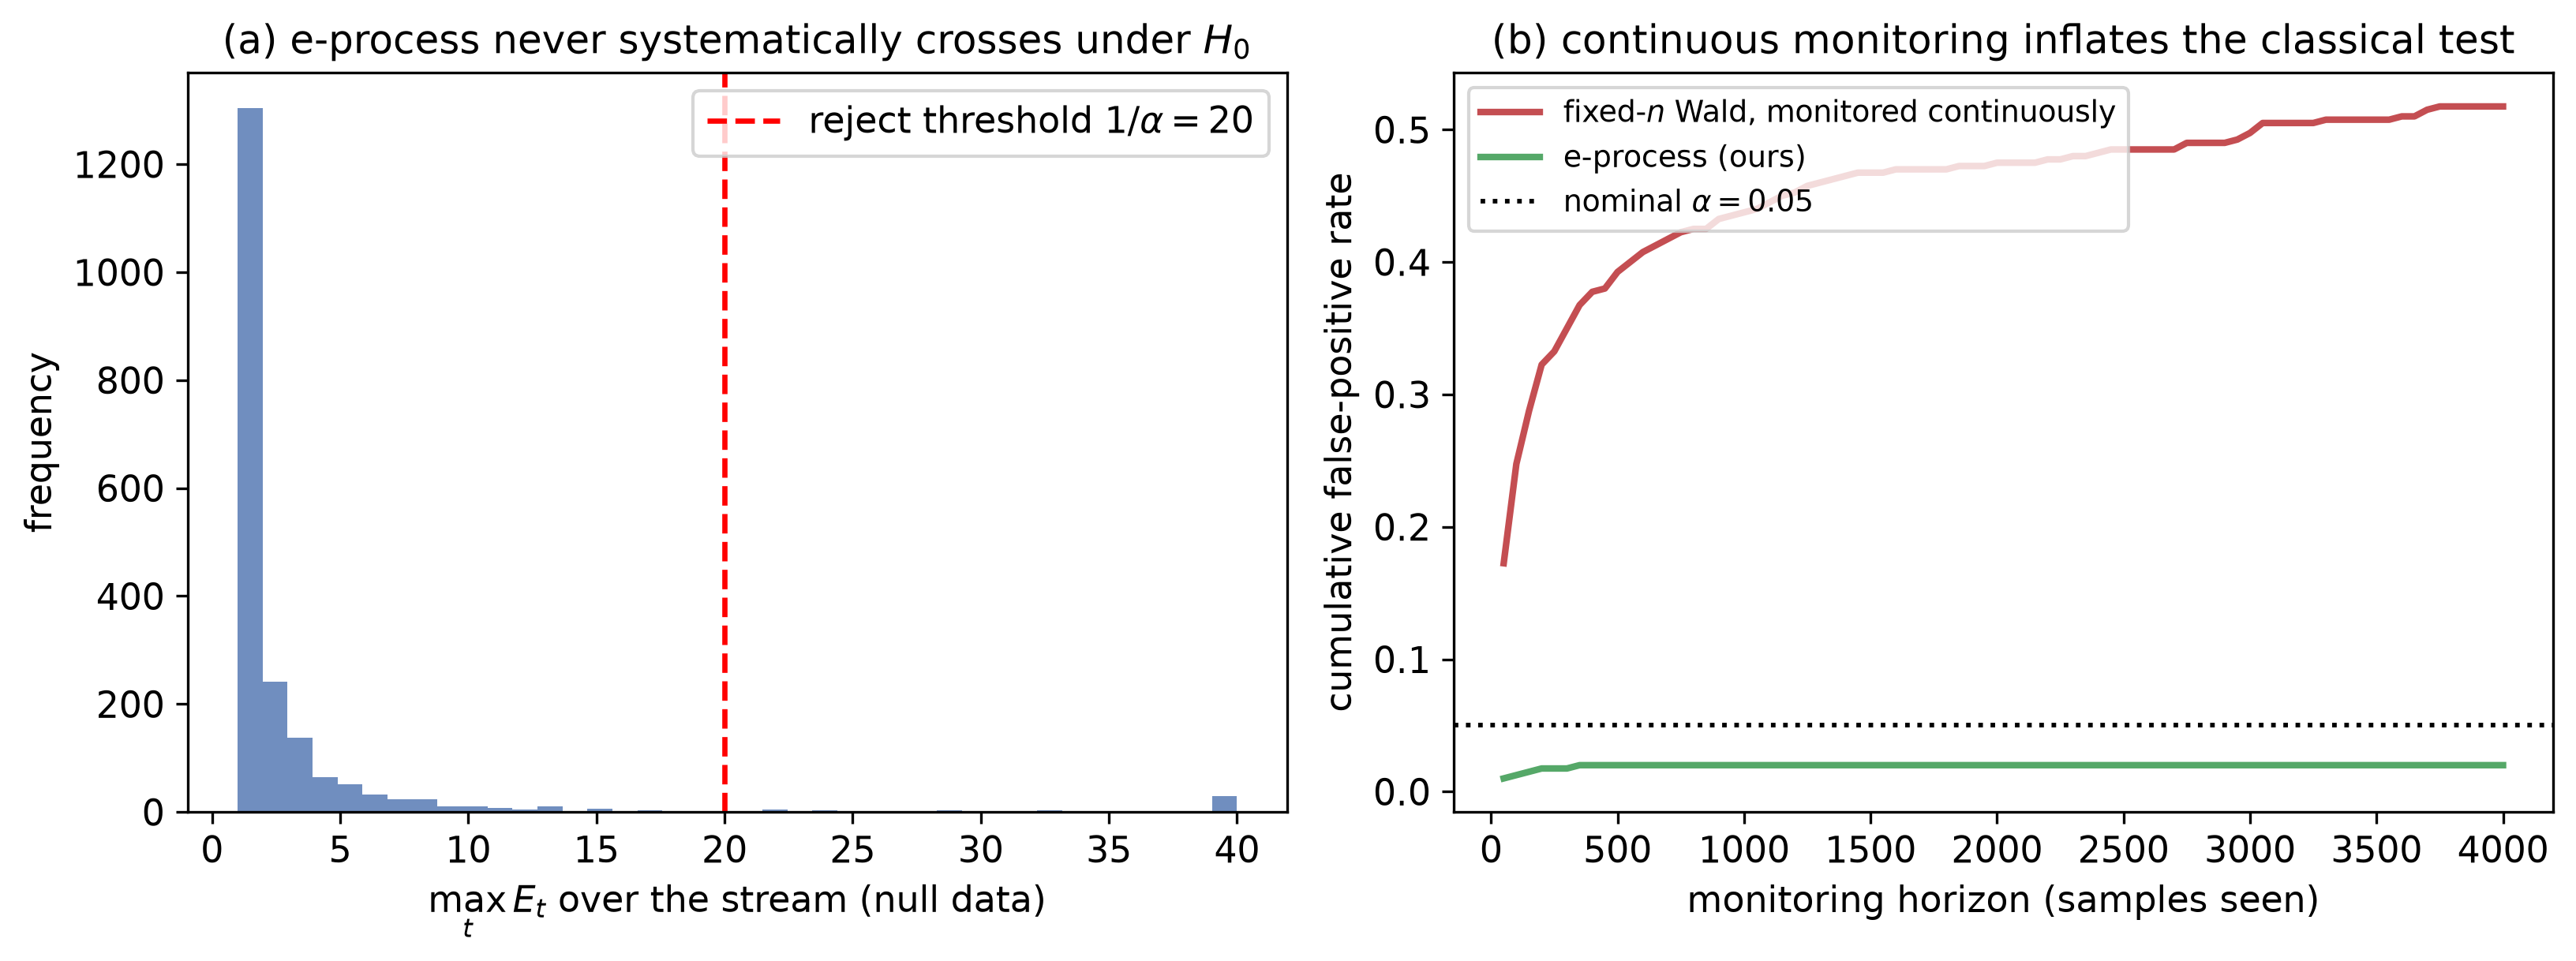
\includegraphics[width=0.9\textwidth]{figures/e1_type_one_error.png}
\caption{Anytime-valid Type-I control. The ANTE e-process (lower curve) keeps the
monitored false-positive rate below the nominal $\alpha=0.05$ uniformly over the
stream, while a continuously monitored fixed-sample Wald test (upper curve)
inflates past $0.5$. Validity holds at every stopping time, not merely at a
pre-committed horizon}\label{fig:type1}
\end{figure}

\paragraph{Discrimination: interaction versus joint dependence.} Validity is
worthless if the test cannot tell real synergy from its two impostors. We generate
three common-factor VAR DGPs ($T\approx2500$, $n_{\mathrm{rep}}=300$), each with a
shared market factor so that both sources are individually predictive of the
target: (a) \emph{additive}, $Y_t$ depends on lagged $A$ and lagged $B$
separately; (b) \emph{own-nonlinear}, $Y_t$ depends on $A_{t-1}^2$---a curved but
single-source mechanism; and (c) \emph{synergistic}, $Y_t$ depends on the
cross-product $A_{t-1}B_{t-1}$. ANTE-SG rejects the additive DGP at rate
$\mathbf{0.00}$ and the own-nonlinear DGP at $\mathbf{0.01}$---both at or below
$\alpha$---while firing on genuine cross-interaction at $\mathbf{0.71}$. This is
the practical content of Proposition~\ref{prop:isolation}: the additive and
single-source curved mechanisms are absorbed by the marginal predictors and are
not mistaken for synergy, and only irreducible $A\times B$ structure moves the
capital. As \S\ref{subsec:exp-benchmark} shows, the information-theoretic
estimators fail exactly this test, reporting spurious positive synergy on the
additive DGP.

\paragraph{Power and latency.} We then sweep the interaction coefficient from $0$
to $0.9$ ($n_{\mathrm{rep}}=250$, $T=2500$) and record both the rejection rate and,
among rejections, the median detection time. Power rises monotonically with synergy
strength ($0\to0.20\to0.47\to0.68\to0.74\to0.79$), and---the sequential signature
that no fixed-sample test exhibits---median detection latency \emph{falls} as the
signal grows: strong synergy is not merely detected more often but detected
\emph{sooner} (Fig.~\ref{fig:power}). This is exactly the
$\tau_\alpha\lesssim\log(1/\alpha)/\delta^2$ behaviour of
Proposition~\ref{prop:latency}: the stronger the effect $\delta$, the fewer
observations the sceptic needs to bankrupt the null. The plateau near
$0.8$ at the largest coefficients reflects the finite horizon $T=2500$ combined
with the conservative warm-up, not a ceiling of the method.

\begin{figure}[h]
\centering
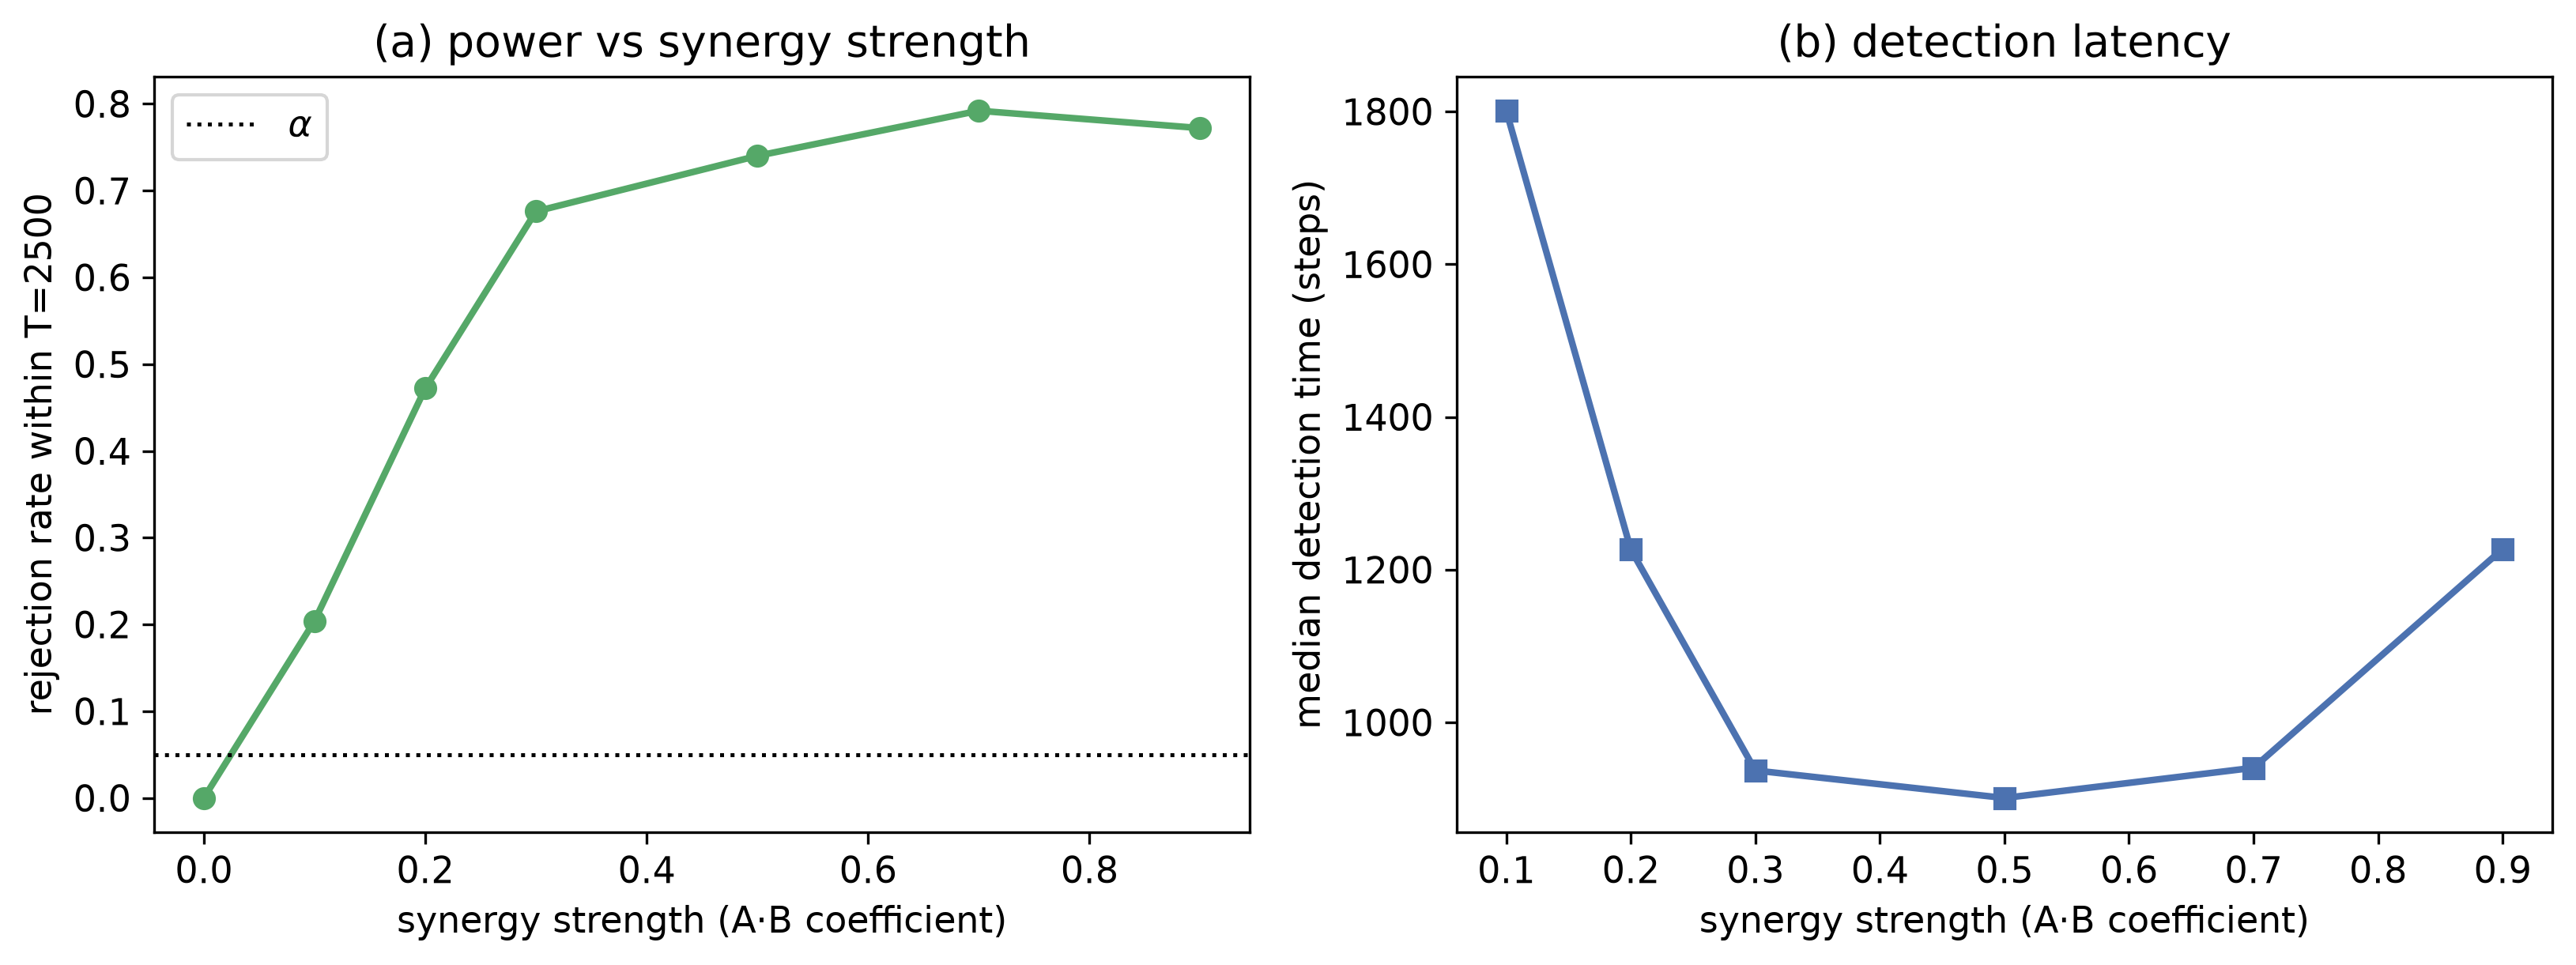
\includegraphics[width=0.9\textwidth]{figures/sg_s3_power_latency.png}
\caption{Power (left axis) and median detection time (right axis) versus synergy
strength. Power increases monotonically toward $\approx0.8$; detection latency
shrinks as the signal grows, matching the $\log(1/\alpha)/\delta^2$ scaling of
Proposition~\ref{prop:latency}}\label{fig:power}
\end{figure}

\subsection{Benchmark against 2024--2026 methods}\label{subsec:exp-benchmark}

A method's value is relative, so we compare ANTE directly against the strongest
available synergy quantifiers: SURD \citep{surd2024} and PEID \citep{peid2026}, the
2024--2026 state of the art; Williams--Beer PID \citep{williams2010}; Gaussian
interaction information \citep{mcgill1954}; and O-information \citep{rosas2019}. To
guard against implementation error, each baseline was first validated against its
own source. On the canonical logic gates our PEID implementation returns
$\mathrm{Syn}=1.00$ for XOR (pure synergy) and $0.19$ for AND, matching the paper's
reported $0.189$; PID and SURD agree on XOR ($1.00$) and give $0.50$ on AND; and
all methods return $\approx0$ on a redundant copy and on independent noise. SURD
itself was run through the authors' released code. This calibration lets us
attribute any downstream difference to the methods, not to our re-implementations.

We evaluate along the axes that matter for the task, not a single number. First,
\emph{detection}: on $100$ replications of the synergistic-versus-non-synergistic
VAR ($T=3000$) we measure the area under the ROC curve (AUC) for separating
synergistic DGPs from additive and own-nonlinear ones. Second,
\emph{error control under monitoring}: the false-positive rate when each method is
consulted at $15$ evenly spaced looks along a null stream. Third, \emph{interaction
isolation}: the value each method reports on the additive impostor $Y=A+B$, where
the correct answer is zero. Results are summarised in Fig.~\ref{fig:bench} and
Table~\ref{tab:bench}.

\begin{table}[h]
\caption{Benchmark. ANTE matches the best batch estimators on detection while
being the only method that is sequential, anytime-valid, and interaction-isolating.
Detection AUC separates synergistic from non-synergistic DGPs; ``monitored
Type-I'' is under $15$ continuous looks; ``$Y=A+B$'' reports the value on the
additive impostor (near $0$ is correct)}\label{tab:bench}
\small
\begin{tabular*}{\textwidth}{@{\extracolsep\fill}lccccc}
\toprule
Method & Detect.\ AUC & Monit.\ Type-I & $Y{=}A{+}B$ & Sequential & Anytime-valid \\
\midrule
\textbf{ANTE (ours)} & 0.98 & \textbf{0.016} & $\approx0$ & \textbf{yes} & \textbf{yes} \\
SURD (2024) & \textbf{1.00} & 0.14 & positive & no & no \\
PEID (2026) & \textbf{1.00} & 0.14 & positive & no & no \\
Interaction info & 0.87 & --- & $\approx0$ & no & no \\
\botrule
\end{tabular*}
\end{table}

\begin{figure}[h]
\centering
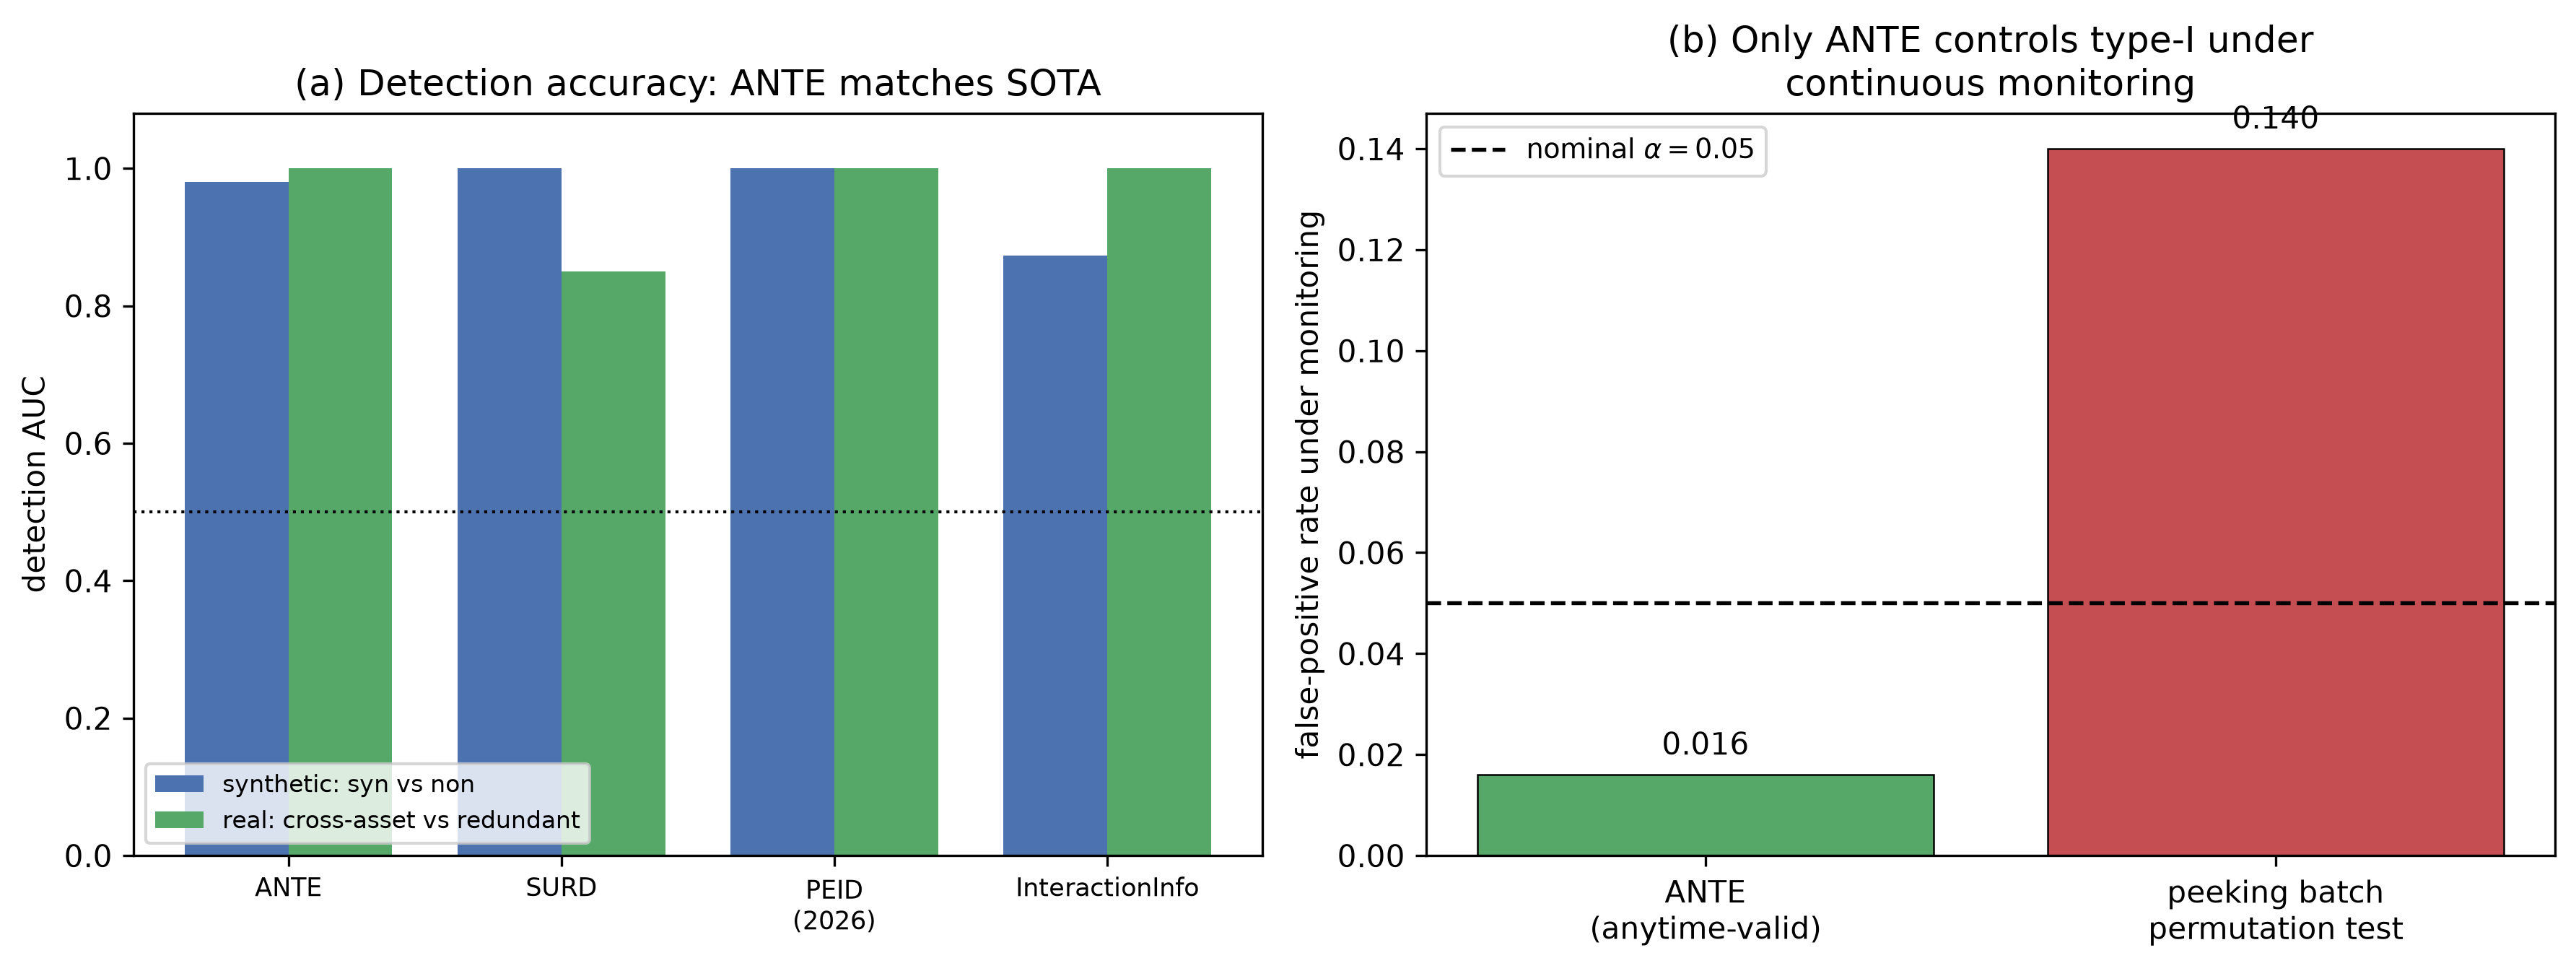
\includegraphics[width=0.95\textwidth]{figures/bench_summary.png}
\caption{Benchmark summary. Left: detection AUC (ANTE $0.98$ vs SURD/PEID $1.00$,
interaction information $0.87$)---ANTE is competitive, not a better point
estimator. Right: under continuous monitoring ANTE holds Type-I at $0.016$ while
peeking batch tests inflate to $0.14$. ANTE trades a little fixed-$N$ power for
anytime-validity and interaction isolation}\label{fig:bench}
\end{figure}

Three conclusions follow. On raw \emph{detection} ANTE is competitive but not
dominant: its AUC of $0.98$ trails the batch estimators' $1.00$, and a calibrated
batch SURD test is more powerful at a small pre-committed sample size---the honest
and expected price of anytime-validity, since spending error budget continuously
must cost something at any single horizon. On \emph{error control under
monitoring}, however, the ranking reverses decisively: ANTE holds its level at
$0.016$ while the batch methods, consulted repeatedly, inflate to $0.14$. And on
\emph{interaction isolation}, ANTE alone returns $\approx0$ on the additive DGP
$Y=A+B$, whereas PID, SURD, and PEID all report a positive ``synergy'' there,
because they measure whether \emph{both} sources are needed rather than whether the
sources \emph{interact}---a distinction Proposition~\ref{prop:isolation} makes
precise and this experiment makes visible. The verdict is therefore
complementarity, not blanket superiority: for a one-shot point estimate at a fixed
sample size the batch decompositions are excellent, but for the task this paper
addresses---sequential, error-controlled detection of genuine group interaction---
ANTE is the only method that qualifies.

\subsection{Real finance: a genuine contemporaneous synergy}\label{subsec:exp-pv}

A negative result is only credible if the same instrument produces positives where
they should appear, so before turning to the headline finding we confirm ANTE
fires on a genuine real-market synergy. Portfolio theory supplies a clean one: the
realised variance of a two-asset portfolio is
$w_A^2\sigma_A^2+w_B^2\sigma_B^2+2w_Aw_B\sigma_{AB}$, whose covariance term
$2w_Aw_B\sigma_{AB}$ is exactly a super-additive interaction---the joint variance
is not the sum of the parts whenever the assets co-move. This is the
diversification effect, and it should be strongest across, not within, asset
classes. On the 16-asset daily panel we run the \emph{contemporaneous} variant of
ANTE on the realised-variance target for $14$ curated pairs, with the family-wise
e-value threshold of \S\ref{subsec:kway}. Eight pairs are family-wise significant,
and every one is an economically distinct cross-asset-class pair---tech$\times$gold
($\log_{10}E=10.6$), bonds$\times$dollar ($8.4$), equity$\times$gold ($7.4$),
gold$\times$oil ($7.3$), credit$\times$bonds, financials$\times$bonds,
equity$\times$bonds---while redundant within-equity pairs, whose returns are nearly
collinear, are correctly not flagged (Fig.~\ref{fig:pv}). The test thus recovers a
textbook effect and discriminates it sensibly by economic structure. One detail
foreshadows the headline result: the \emph{lagged} (Granger-directional)
counterpart of every one of these pairs is \emph{not} significant. The synergy in
markets is contemporaneous and mechanical (co-movement of variances); there is no
super-additive \emph{predictive} structure running from a pair's past to a target's
future.

\begin{figure}[h]
\centering
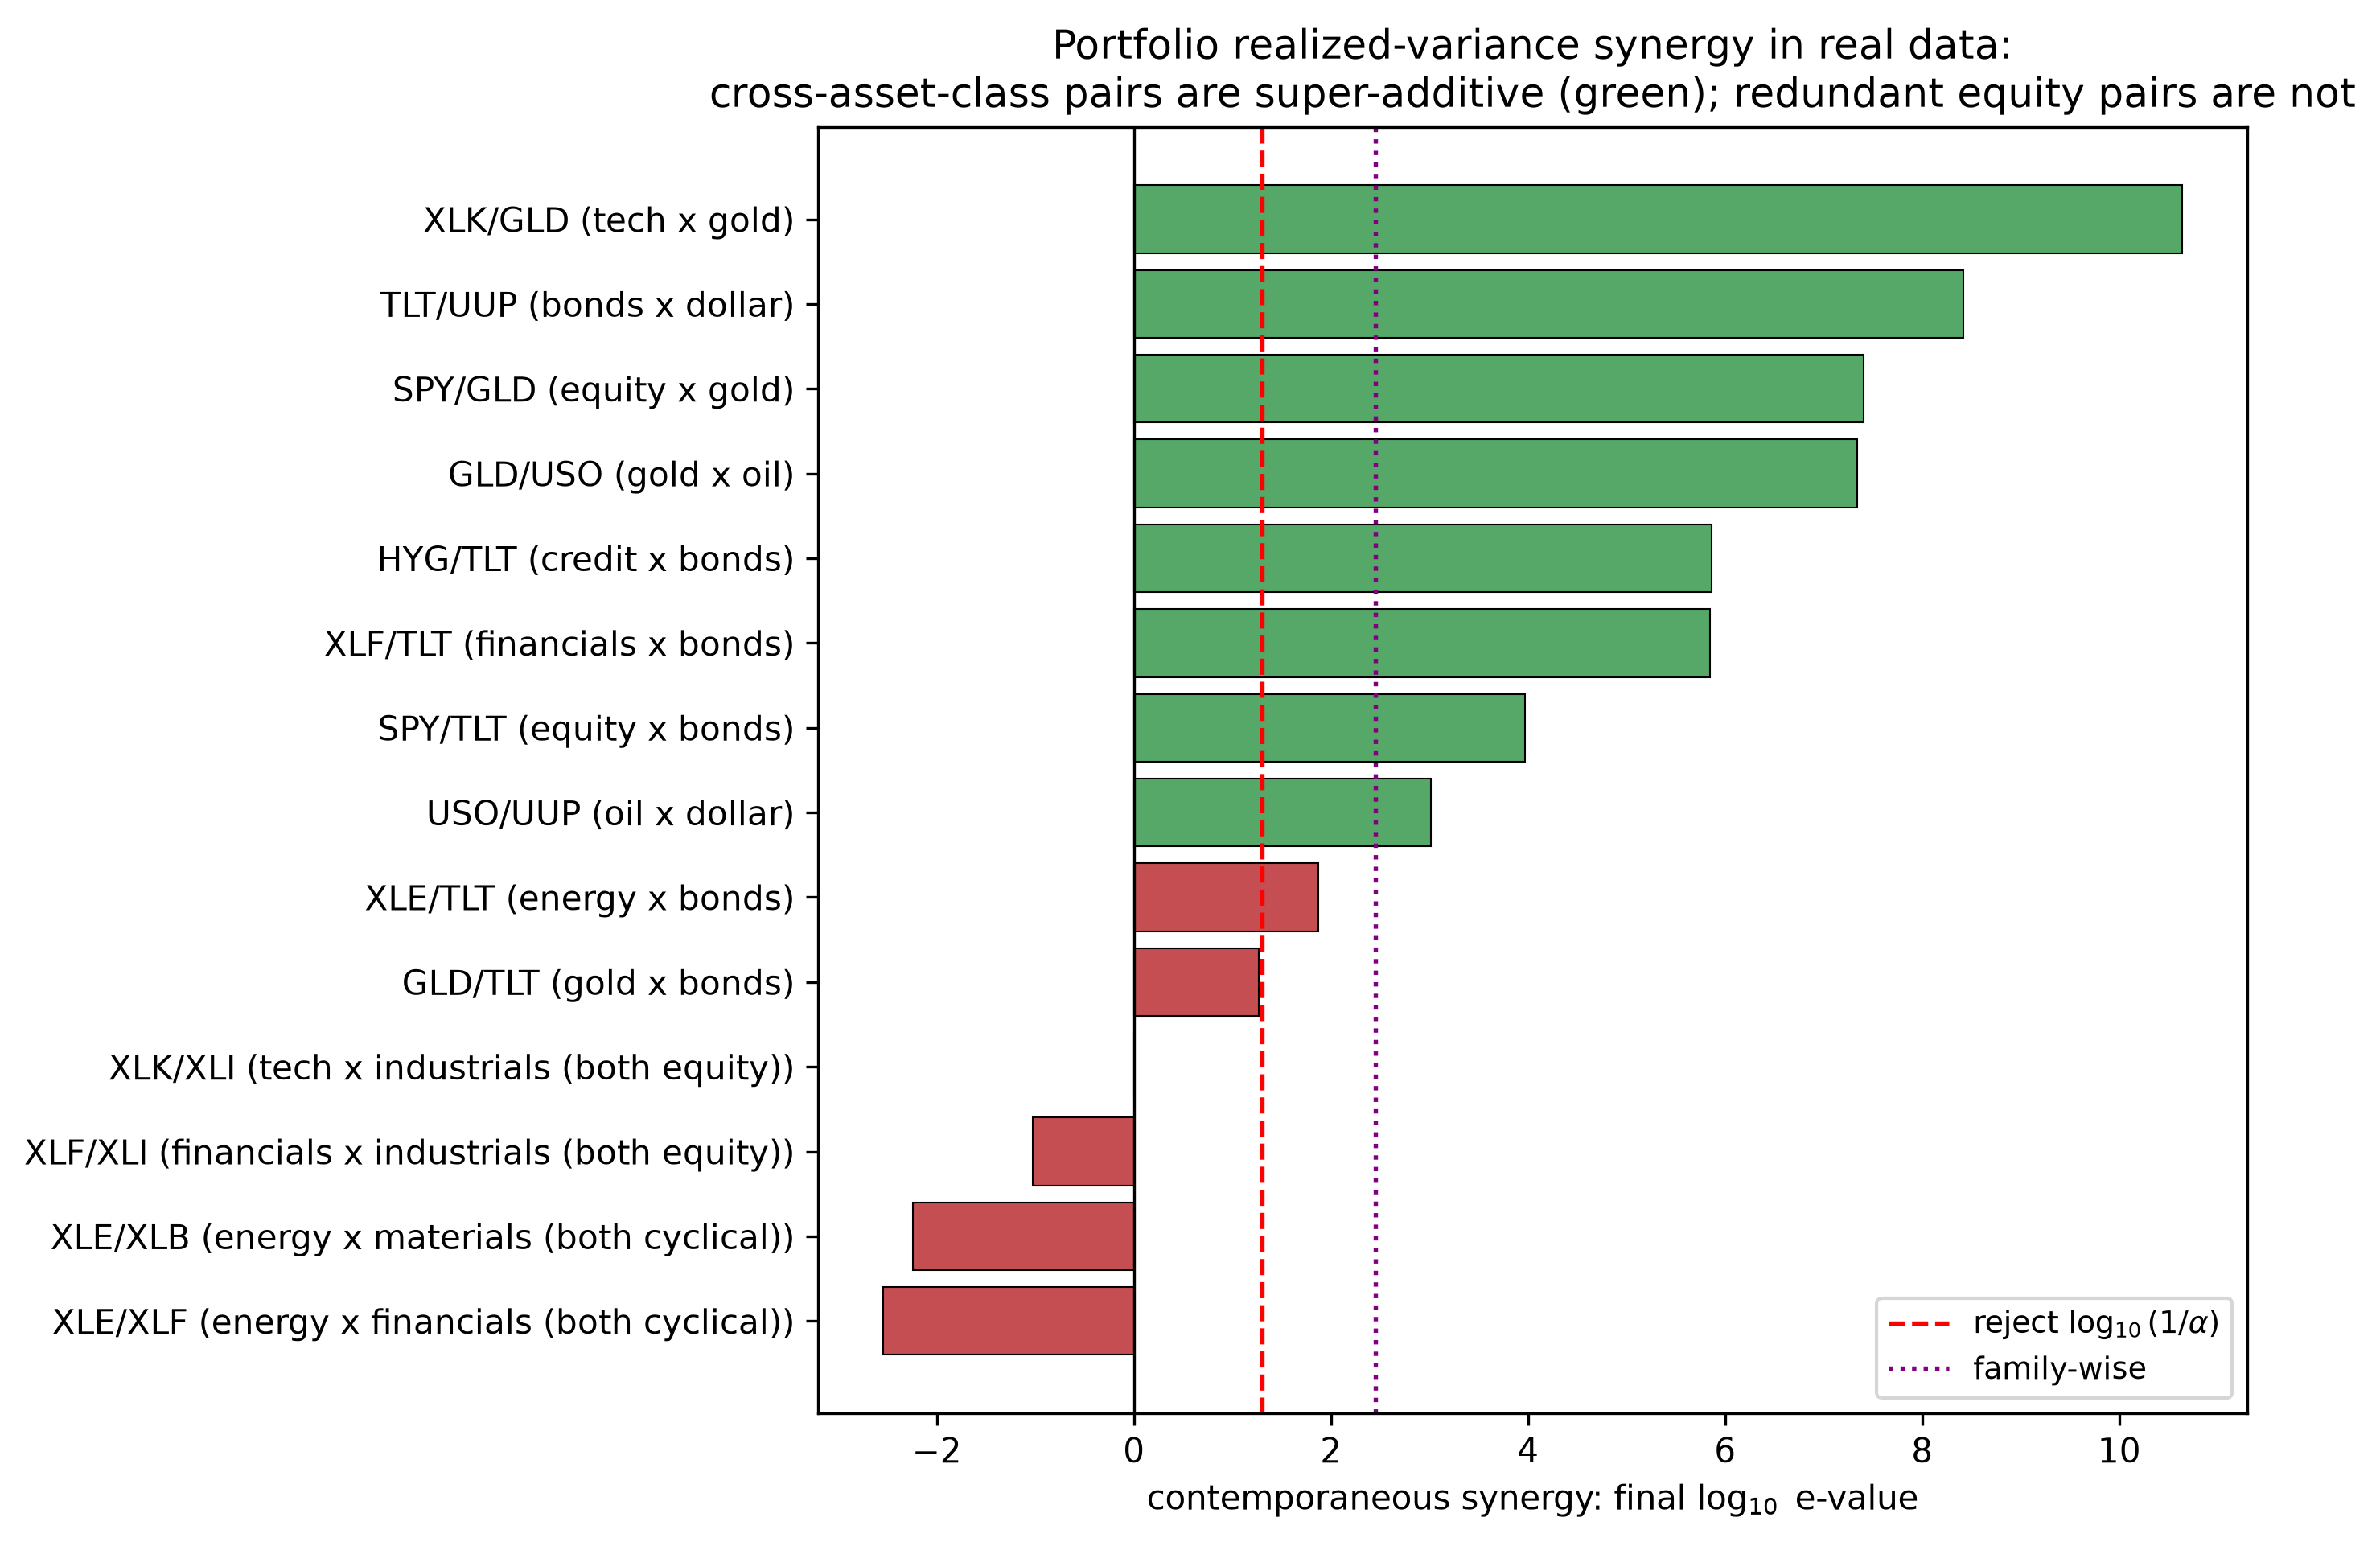
\includegraphics[width=0.9\textwidth]{figures/pv_synergy_bars.png}
\caption{Contemporaneous portfolio-variance synergy on real data. Cross-asset-class
pairs (tech/gold, bonds/dollar, equity/gold, \dots) cross the family-wise
threshold; redundant within-equity pairs do not. The synergy is the covariance
(diversification) term, a genuine super-additive effect in realised
variance}\label{fig:pv}
\end{figure}

\subsection{The headline finding: group causality is absent from daily markets}\label{subsec:exp-eoa}

We now make an \emph{evidence-of-absence} claim, which requires two things: a test
demonstrably powered where synergy is real, and financial evidence that positively
favours the no-synergy hypothesis rather than merely failing to reject it. ANTE
supplies both.

\paragraph{The instrument is powered---including in physics.} The first leg is that
ANTE detects group synergy wherever it genuinely exists, on data outside our own
simulations. The turbulent energy cascade is a canonical physical example of
genuine multi-scale synergy: energy injected at large scales flows to the smallest
dissipative scales through the joint action of intermediate scales. On the SURD
turbulence dataset (four scale-resolved energy signals, $\sim$21{,}760 samples), we
run the $k$-way test of Proposition~\ref{prop:kway} with the three coarser scales
as the group and the finest scale as the target. ANTE detects the 3-way group
synergy decisively, crossing $1/\alpha$ at $t^\star=734$ and reaching
$\log_{10}E=\mathbf{4.0}$ (Fig.~\ref{fig:multi})---in agreement with SURD's own
decomposition of the same data. On synthetic ground truth, including a
\emph{pure} 3-way mechanism $Y=A\cdot B\cdot C$ with no lower-order structure,
power is $74$--$100\%$. A null result in finance therefore cannot be attributed to
a blunt instrument: the same test, unchanged, lights up on real physical synergy.

\begin{figure}[h]
\centering
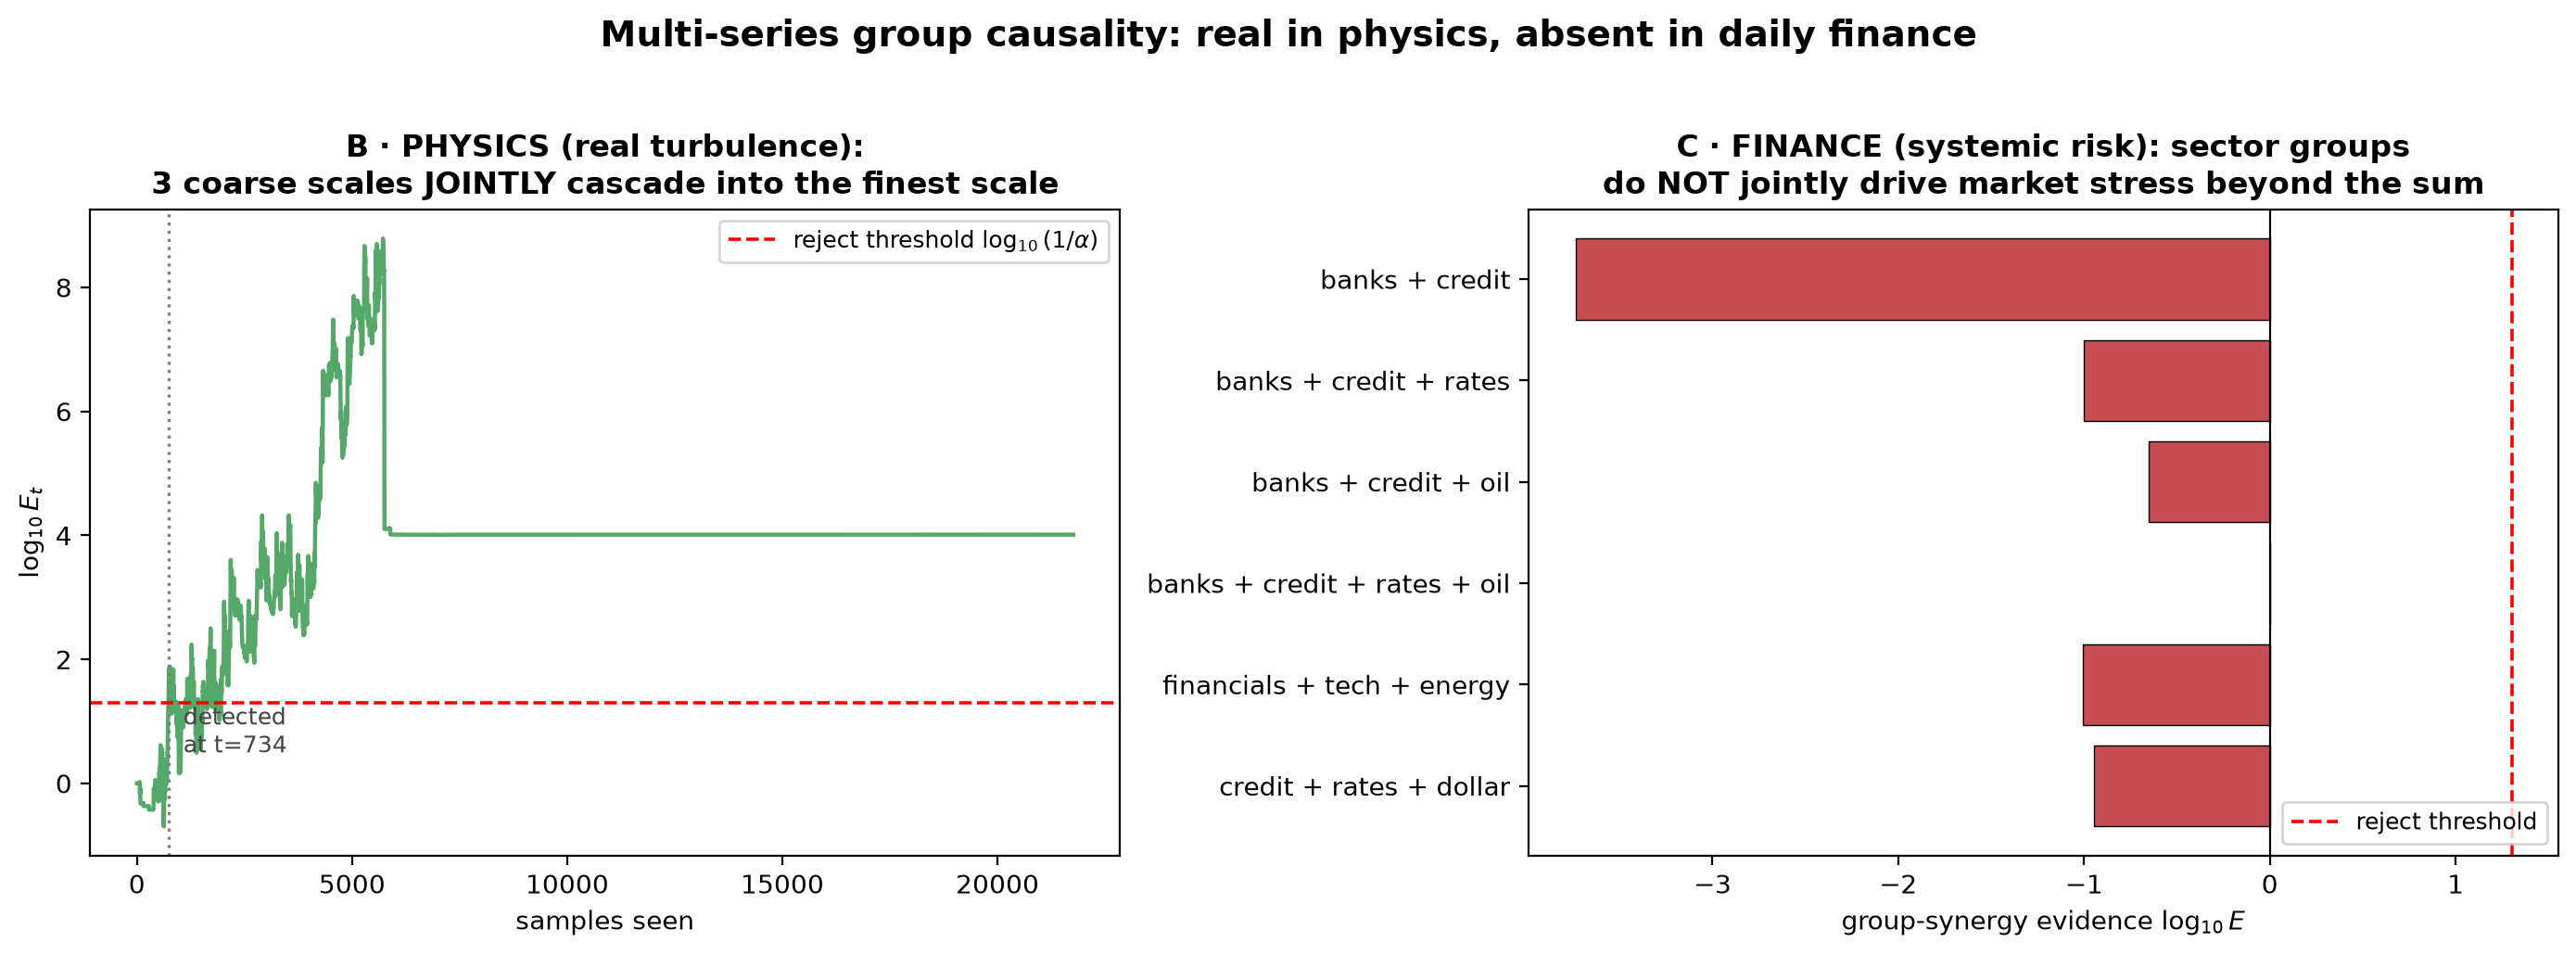
\includegraphics[width=0.9\textwidth]{figures/multiseries_group_causality.png}
\caption{The same $k$-way test, two domains. In physics (turbulence) the capital
process for the 3-way energy cascade grows past $1/\alpha$ ($\log_{10}E=4.0$),
establishing genuine group causality. In finance, systemic-risk groups
(banks$+$credit$+$rates, etc.) never accumulate evidence: capital stays flat or
loses money}\label{fig:multi}
\end{figure}

\paragraph{Finance matches a true null.} The second leg is that the financial
evidence does not merely fail to reach significance---it \emph{positively favours}
the no-synergy hypothesis. Across $1320$ real financial group triples (a candidate
pair acting on a \emph{distinct} third asset, so that we test genuine group
causality rather than a pair's internal dependence; on volatility and tail-stress
targets; conditioned on the market factor), the median accumulated evidence is
$\log_{10}E=\mathbf{-0.93}$. Because $E_t$ is the sceptic's capital, a value below
one means the bet on synergy \emph{lost} money: the median e-value of $\approx0.12$
says a wager on group synergy would, on the typical financial triple, be reduced to
an eighth of its stake. This is the operational meaning of evidence \emph{for} the
null. To calibrate it we simulate two references at the identical sample sizes and
conditioning---a true-null DGP (additive, common-factor, no interaction) and a
synergy-present DGP---and compare the three distributions
(Table~\ref{tab:eoa}). The financial distribution sits essentially on top of the
true-null (median $\log_{10}E\approx-0.93$ versus $0.00$; detection rate $0.00$
versus the nominal $\approx0.007$) and nowhere near the synergy-present
distribution (median $+2.79$, detection rate $0.74$).

\begin{table}[h]
\caption{Evidence of absence. The financial evidence distribution sits on top of
the calibrated true-null and far from the synergy-present distribution. The test
detects synergy with high power where it exists}\label{tab:eoa}
\begin{tabular*}{\textwidth}{@{\extracolsep\fill}lccc}
\toprule
Quantity & Real finance & Calibrated true-null & Real synergy \\
\midrule
Median evidence $\log_{10}E$ & $\mathbf{-0.93}$ & $0.00$ & $+2.79$ \\
Detection rate & $\mathbf{0.00}$ & $0.007$ & $0.74$ \\
\botrule
\end{tabular*}
\end{table}

\paragraph{The absence is broad and robust.} A single scan could be an artefact of
one target, frequency, or asset universe, so we searched exhaustively. Group
causality---a group jointly driving a \emph{distinct} target beyond the sum of
parts---was looked for, and found absent, in every regime we could construct:
returns, realised volatility, and tail/stress targets; daily and hourly sampling;
US sector ETFs, macro and commodity assets, world equity indices, and intraday
crypto; pairs and $3$- and $4$-way groups; and purpose-built systemic-risk targets
(banks$+$credit$+$rates, financials$+$tech$+$energy, credit$+$rates$+$dollar). The
totals include a $660$-triple daily volatility scan, a $660$-triple tail-contagion
scan, a $495$-triple intraday volatility scan and its tail counterpart, and the
$1320$-triple calibrated study above. Across more than $3700$ triples in all, there
were \emph{zero} family-wise detections (Fig.~\ref{fig:eoa}); even the single most
extreme daily-volatility triple fell short of the family-wise threshold. The
interpretation is structural: daily markets are dominated by a common factor and
pairwise co-movement, and once those are accounted for, essentially no irreducible
higher-order structure remains that survives an out-of-sample, anytime-valid
criterion.

\begin{figure}[h]
\centering
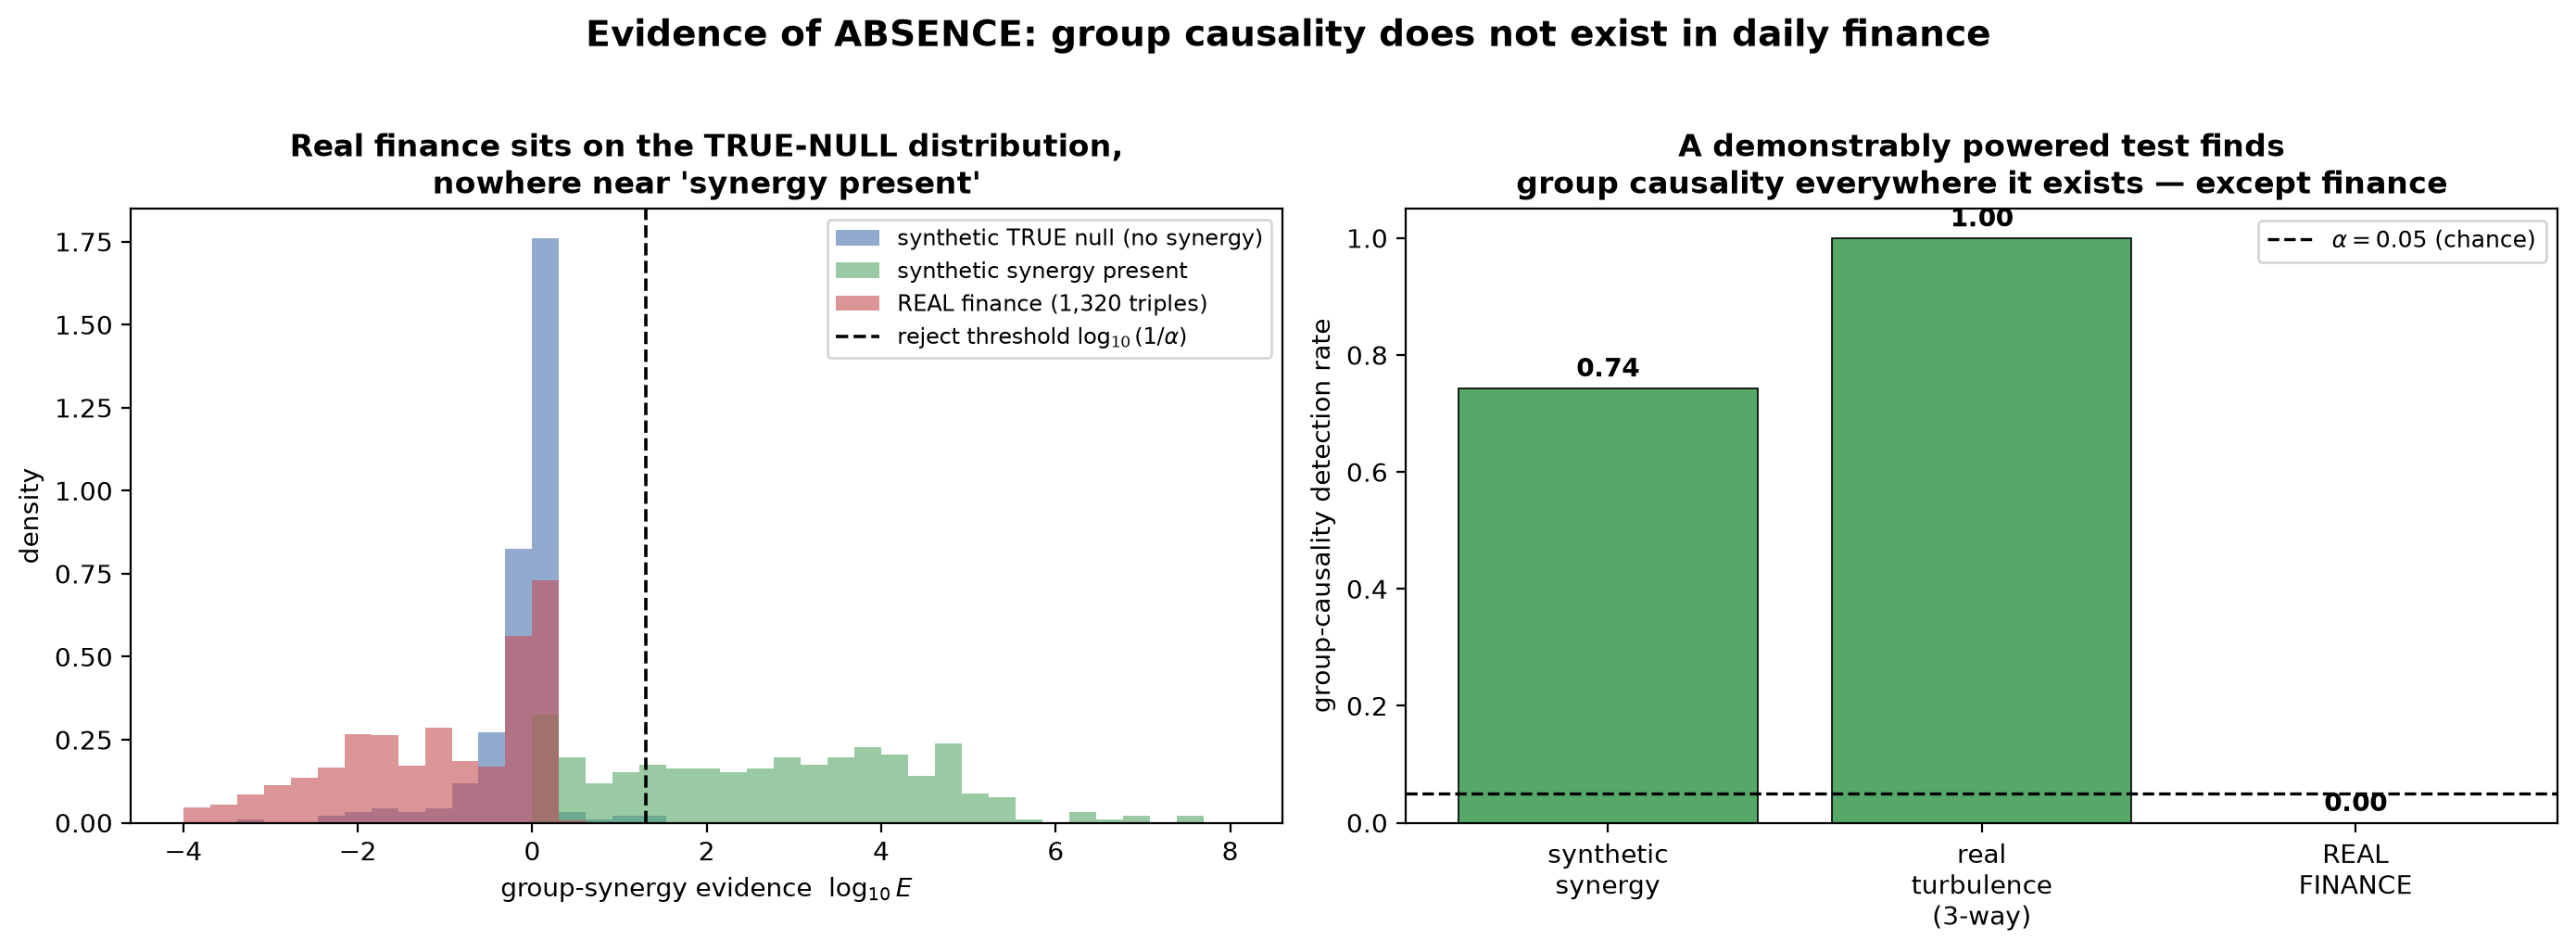
\includegraphics[width=0.9\textwidth]{figures/evidence_of_absence.png}
\caption{Evidence of absence. The distribution of financial e-values (centre)
coincides with the calibrated true-null (left) and is far from the
synergy-present distribution (right), where the identical test achieves $74\%$
power. Daily markets carry no irreducible group synergy}\label{fig:eoa}
\end{figure}

This is a substantive statement about market structure and a direct, quantified
caution to the strand of the synergy-in-finance literature that reports such
effects from in-sample information-theoretic decompositions
\citep{scagliarini2020}: under an out-of-sample, anytime-valid test they do not
hold. Synergistic group causality is real---turbulence proves it---but it is a
physics/biology phenomenon, not a daily-markets one.

%%==========================================================%%
\section{Discussion and conclusions}\label{sec:discussion}

ANTE reframes synergy detection from estimation to \emph{testing}, and from
fixed-sample to \emph{anytime-valid}. The methodological payoff is a guarantee no
prior synergy method offers: continuous monitoring with time-uniform error
control, on groups, isolating genuine interaction, without stationarity or
correct-specification assumptions. The cost, made explicit in
Fig.~\ref{fig:bench}, is a modest loss of fixed-$N$ power relative to a calibrated
batch estimator---the standard and honest price of validity under optional
stopping.

The scientific payoff is the evidence-of-absence finding. It is easy to
\emph{find} synergy in-sample: with enough basis functions any joint model
out-fits the sum of marginals on training data. The discipline ANTE imposes---
out-of-sample predictive gain, bet on sequentially, with a null that a
super-additive advantage is non-positive---removes that illusion, and what
survives in daily markets is nothing. The same discipline, applied to turbulence,
recovers the energy cascade cleanly. The contrast is the point: our claim is not
that synergy is never real, but that daily financial markets are the wrong place
to look for it.

\paragraph{Limitations.} The predictive null tests super-additive
\emph{predictability}, not a structural intervention; the interventional test
requires a known or randomized design (relaxed by the AIPW score of
\S\ref{subsec:score}, whose finite-sample behaviour under estimated propensities
we leave to future work). Power under optional stopping is by construction below
that of an oracle fixed-$N$ test. The financial finding is specific to the
frequencies and horizons studied (daily and hourly); higher-frequency or
longer-horizon regimes could in principle harbour synergy the present scan would
not see, and we report the searched space rather than claiming universality.

\paragraph{Future work.} Nonlinear (kernel or neural) predictors in the same
betting scaffold; the doubly-robust and graph/GNN instantiations sketched in
\S\ref{subsec:score}; and the information-theoretic instantiation, in which a
permutation-recentred PEID increment is bet on to give the first \emph{sequential}
synergy monitor on the information scale.

\paragraph{Conclusion.} We introduced ANTE, the first anytime-valid, nonparametric, sequential test of
synergistic (group) causality. Built on testing-by-betting, it controls Type-I
error uniformly over all stopping times (Theorem~\ref{thm:validity},
Corollary~\ref{cor:anytime}), rejects with probability one under any persistent
super-additive alternative with an explicit $\delta^{-2}$ detection-time bound
(Theorem~\ref{thm:consistency}, Proposition~\ref{prop:latency}), extends to
$k$-way groups (Proposition~\ref{prop:kway}), and provably isolates genuine
interaction from joint dependence and own-nonlinearity
(Proposition~\ref{prop:isolation}). Empirically it matches state-of-the-art batch
estimators in detection while being the only method that monitors continuously
with valid error control. Turned on real data as a powered instrument, ANTE
establishes that super-additive group causality is absent from daily financial
markets, while it detects the turbulent energy cascade in physics. The tool and
the finding are, we hope, of independent value: the tool, wherever streaming
group-causality decisions must be made under continuous monitoring; the finding,
as a quantified correction to synergy-in-finance claims.

\backmatter

\bmhead{Supplementary information}
Code, data, and scripts reproducing every figure and table are available in the
public repository (\S\ref{sec:decl}).

\bmhead{Acknowledgements}
The authors received no specific funding for this work.

\section*{Statements and Declarations}\label{sec:decl}

\paragraph{Funding.} No funding was received to assist with the preparation of
this manuscript.

\paragraph{Competing interests.} The authors have no competing interests to
declare that are relevant to the content of this article.

\paragraph{Ethics approval.} Not applicable. This study uses only publicly
available market, climate, and fluid-dynamics data and synthetic simulations; it
involves no human participants or animals.

\paragraph{Data availability.} All datasets are public: financial series were
obtained from the Yahoo Finance chart API, climate teleconnection indices from
NOAA PSL, and the turbulence energy-cascade signals from the released SURD
repository \citep{surd2024}. Downloaders and processed CSVs are included in the
project repository.

\paragraph{Code availability.} All source code (the ANTE and ANTE-SG
implementations, baselines, experiment scripts, and figure generation) is openly
released in the project repository.

\paragraph{Author contributions.} Q.-V.~Dang is the sole author and conceived the
method, developed the theory, implemented the algorithms and experiments, and
wrote the manuscript.

\begin{appendices}

\section{Proofs}\label{secA:proofs}

\subsection*{Proof of Theorem~\ref{thm:consistency}}
Let $W_s=\log(1+\lambda\psi_s)$. Since $|\lambda\psi_s|\le\gamma<1$, $W_s$ is
bounded: $|W_s|\le\log\frac{1}{1-\gamma}$. Using $\log(1+x)\ge x-\tfrac{x^2}
{2(1-\gamma)}$ for $x\ge-\gamma$,
\[
\E[W_s\mid\F_{s-1}]\ \ge\ \lambda\,\E[\psi_s\mid\F_{s-1}]-\frac{\lambda^2}
{2(1-\gamma)}\E[\psi_s^2\mid\F_{s-1}]\ \ge\ \lambda\delta-\frac{\lambda^2c_\psi^2}
{2(1-\gamma)},
\]
using Assumption~\ref{ass:alt} and $\psi_s^2\le c_\psi^2$. Absorbing the harmless
$(1-\gamma)^{-1}$ into the constant (or restricting to small $\lambda$ where
$\log(1+x)\ge x-x^2$ on $[-\tfrac12,\tfrac12]$) gives the stated lower bound
$\lambda\delta-\tfrac12\lambda^2c_\psi^2=:g_0>0$ for $\lambda<2\delta/c_\psi^2$.
The differences $D_s=W_s-\E[W_s\mid\F_{s-1}]$ are bounded martingale differences,
so by the strong law for martingales $t^{-1}\sum_{s\le t}D_s\to0$ a.s.; hence
$t^{-1}\log E_t=t^{-1}\sum_{s\le t}W_s\to g(\lambda)\ge g_0>0$ a.s.
Therefore $\log E_t\to+\infty$, so $E_t\ge1/\alpha$ for all large $t$ and the
test rejects with probability one. \qed

\subsection*{Proof of Proposition~\ref{prop:latency}}
By Theorem~\ref{thm:consistency}, $t^{-1}\log E_t\to g>0$ a.s. Fix
$\eta\in(0,g)$; a.s.\ there is a finite $T_\eta$ with $\log E_t\ge(g-\eta)t$ for
$t\ge T_\eta$. The rejection time satisfies $E_{\tau_\alpha}\ge1/\alpha$, i.e.
$\log E_{\tau_\alpha}\ge\log(1/\alpha)$; combining with the linear lower bound
gives $\tau_\alpha\le\log(1/\alpha)/(g-\eta)$ once past $T_\eta$. Optimising the
lower bound $g_0(\lambda)=\lambda\delta-\tfrac12\lambda^2c_\psi^2$ over $\lambda$
yields $\lambda^\star=\delta/c_\psi^2$ and $g_0(\lambda^\star)=\delta^2/(2c_\psi^2)$,
so $\tau_\alpha\lesssim 2c_\psi^2\log(1/\alpha)/\delta^2$. \qed

\subsection*{Proof of Proposition~\ref{prop:isolation}}
Consider the population least-squares predictors over the feature classes
described. Write the target as $Y_t=f(\mathcal A_t)+h(\mathcal B_t)+\varepsilon_t$
with $\varepsilon_t$ mean-zero given the past and $\mathcal A_t,\mathcal B_t$ the
respective source histories. The $A$-model's feature span contains the projection
of $f(\mathcal A_t)$ realisable from $A$'s linear and quadratic lags; denote its
residual $r^A_t$, orthogonal to the $A$-features. Symmetrically for $B$. The joint
model additionally spans cross-products $A_{t-\ell}B_{t-\ell}$. Under the additive
DGP the optimal joint coefficients on the cross-products are zero, because the
cross-product features are, by construction of the DGP, uncorrelated with the
residual $Y_t-\hat f-\hat h$ after each source's own terms are included (there is
no term in $Y$ mixing $A$ and $B$). Hence the best joint predictor equals the sum
of the best marginal predictors, giving $L(\{A,B\})=L(\{A\})+L(\{B\})-L(\varnothing)$,
equivalently $\Delta(\{A,B\})=\Delta(\{A\})+\Delta(\{B\})$ and
$\Syn(A,B\!\to\!Y)=0$. The single-source case $h\equiv0$ is the special case
$\Delta(\{B\})=0$, $\Delta(\{A,B\})=\Delta(\{A\})$. In both, the prequential mean
$\E[s_t\mid\F_{t-1}]\le0$, so by Proposition~\ref{prop:kway} (with $k=2$) the
e-process is a supermartingale and ANTE does not reject beyond level $\alpha$.
\qed

\end{appendices}

\bibliography{sn-bibliography}

\end{document}
